\documentclass[DIV=13, 10pt,a4paper]{scrartcl}


\usepackage[utf8]{inputenc}
\usepackage[ngerman]{babel}
\usepackage{eurosym}
\usepackage{geometry}
\usepackage{xcolor,colortbl}
\usepackage{graphicx}
\usepackage[headsepline,footsepline,automark]{scrpage2}
\usepackage{pdfpages}
\usepackage{tabularx}
\usepackage{tabulary}
\usepackage{multicol}
\usepackage{multirow}
\usepackage{amssymb}
\usepackage{amsmath}
\usepackage{color, colortbl}
\usepackage{lscape}
\usepackage[toc,page]{appendix} 
\usepackage{caption}
\usepackage{hyperref}


\usepackage{lipsum}% Used for dummy text.

\newlength{\mylength}
\setlength{\mylength}{\textwidth}
\addtolength{\mylength}{-\parindent}

\definecolor{titlepagecolor}{cmyk}{1,.60,0,.70}
\definecolor{namecolor}{cmyk}{0,.24,.07,.47} 

\makeatletter                       
\def\printauthor{%                  
	{\small \@author}}   
	\renewcommand{\@dotsep}{10000}            
\makeatother

\author{%
	Patrick Gruber
	\texttt{\mailto{patrick.gruber@st.oth-regensburg.de}}\vspace{10pt} \\
	Markus Bauer 
	\texttt{\mailto{ markus.bauer@st.oth-regensburg.de}}\vspace{10pt} \\
	Marius Tuschl
	\texttt{\mailto{ marius.tuschl@st.oth-regensburg.de}}\vspace{10pt} \\
	Richard Tscharntke
	\texttt{\mailto{richard.tscharntke@st.oth-regensburg.de}}
}

\pagestyle{scrheadings}
\cfoot[]{}
\ofoot[]{\pagemark}
\setkomafont{pageheadfoot}{\normalfont\sffamily}

\newcommand{\colorcell}[1]{\cellcolor{namecolor}\color{white}\textbf{#1}}
\newcommand{\colorcelllight}[1]{\cellcolor{namecolor!25}\color{black}{#1}}
\newcommand{\mailto}[1]{\href{mailto:#1}{#1}}

%-----------------------------------------------------------------
\begin{document}
% ----------------------------------------------------------------
\begin{titlepage}

\newgeometry{left=3cm,right=4cm} %defines the geometry for the titlepage
\pagecolor{titlepagecolor}
\noindent

\includegraphics[width=3cm]{docs/0_Sonstiges/logo/poppal_white.png}\\[1em]
\color{white}
{\LARGE \textbf{\textsf{PPP - Pen\&Paper Pal}}}\\
\makebox[0pt][l]{\rule{1.3\textwidth}{1pt}}
\par
\noindent
\textbf{\textsf{Ostbayrische Technische Hochschule}} \textcolor{namecolor!25}{\textsf{Regensburg}}
\vfill
\noindent
\begin{minipage}[t]{0.35\linewidth}
	\vspace{0pt}
	\begin{flushleft}
		\printauthor
	\end{flushleft}
\end{minipage}
%\hspace{15pt}
\hfill
\begin{minipage}[t]{0.5\linewidth}
	\vspace{40pt}
	{\huge \textsf{Projektbericht}}
	\vskip\baselineskip
	\noindent
	\textsf{\today}
\end{minipage}
\end{titlepage}
\restoregeometry % restores the geometry
\nopagecolor% Use this to restore the color pages to white
% ----------------------------------------------------------------

\tableofcontents
\thispagestyle{empty}
\pagebreak
\setcounter{page}{1}

\section{Projektvision}
\thispagestyle{empty}
	\begin{flushleft}
		
\includegraphics[page=1,width=0.75\textwidth]{docs/0_Sonstiges/PNrot.pdf}
		\vfill
	\end{flushleft}
	\begin{center}
		
\includegraphics[page=2,width=0.75\textwidth]{docs/0_Sonstiges/PNrot.pdf}
		\vfill
	\end{center}
	\begin{flushright}
		
\includegraphics[page=3,width=0.75\textwidth]{docs/0_Sonstiges/PNrot.pdf}
	\end{flushright}

\section{Projektauftrag}
\begin{tabularx}{\textwidth}{|c|X|}
	\hline
	\colorcell{Projekttitel} & PPP - Pen\&Paper Pal\\
	\hline
\end{tabularx}
\newline
\vspace{2pt}
\newline
\begin{tabularx}{\textwidth}{|l|X|l|X|}
	\hline
	\multicolumn{4}{|l|}{\colorcell{Projektdaten}}\\
	\hline
	\colorcelllight{Start} & 28.03.2018 & \colorcelllight{Projektkategorie} & Kleinprojekt\\
	\cline{2-2} \cline{4-4}
	\colorcelllight{Ende} & 10.07.2018 & \colorcelllight{Projektnummer} & 420\\
	\hline
\end{tabularx}
\newline
\vspace{2pt}
\newline
\begin{tabularx}{\textwidth}{|l|X|l|X|}
	\hline
	\multicolumn{4}{|l|}{\colorcell{Projektorganisation}} \\
	\hline
	\colorcelllight{Projektmanager*in} & Markus Bauer & \colorcelllight{Projektauftraggeber*in} & Carsten Kern\\
	\cline{2-4}
	\colorcelllight{} &\multicolumn{1}{l}{Patrick Gruber}& \multicolumn{1}{l}{Richard Tscharntke}  & \\
	\multirow{-2}{*}{\colorcelllight{Projektteammitglieder}}& \multicolumn{1}{l}{Marius Tuschl} & \multicolumn{1}{l}{Markus Bauer}& \\
	\hline
\end{tabularx}
\newline
\vspace{2pt}
\newline
\begin{tabularx}{\textwidth}{|l|X|}
	\hline
	\multicolumn{2}{|l|}{\colorcell{Projektbeschreibung}}\\
	\hline
	\colorcelllight{Projektbegründung} & Es ist aufwendig Mitspieler für Gesellschaftsspiele zu finden.\\
	\cline{2-2}
	\colorcelllight{Projektgesamtziel} & Entwicklung und Deployment eines sozialen Netzwerkes zur Suche und Organisation von Mitspielern für Gesellschaftsspiele. Der Zugriff auf das Netzwerk erfolgt über eine mobile Applikation auf den aktuellen Android Versionen.\\
	\hline
	\multicolumn{1}{|l}{\colorcell{Projektteilziele $\Rightarrow$}} & \multicolumn{1}{l|}{\colorcell{Messbare Ergebnisse}}\\
	\hline
	Backend & Funktionalitäten können über API verwendet werden.\\
	\cline{2-2}
	Anmeldung & User können  einn Profil erstellen.\\
	\cline{2-2}
	Suche & User können andere User finden.\\
	\cline{2-2}
	Filter & User können nach Spiel, Ort, Datum, durchschnittlichem Alter und Geschlecht filtern.\\
	\cline{2-2}
	Bewertung & User können andere User und Spiele anhand verschiedener Kriterien bewerten.\\
	\cline{2-2}
	Gruppen & User können sich in Gruppen zusammenschließen, per Chat unterhalten und mit einem Kalender gemeinsame Termine verwalten.\\
	\cline{2-2}
	Tauschbörse & User können auf einer Tauschbörse Spiele im Tausch gegen andere Spiele suchen und anbieten. \\
	\cline{2-2}
	Forum & User können in einem für jeden User zugänglichen Forum Informationen austauschen.\\
	\cline{2-2}
	Werbeintegration & In unserer App kann über ADSense Werbung geschalten werden.\\
	\hline
	\colorcelllight{Nicht-Ziele} & Exklusion\\
	\cline{2-2}
	\colorcelllight{Wirkung/Nutzen} & Inklusion.\\
	\hline
	\colorcelllight{} & 1. Backend implementieren.\\
	\cline{2-2}
	\colorcelllight{} & 2. Fronntend implementieren.\\
	\cline{2-2}
	\colorcelllight{} & 3. Testen.\\
	\cline{2-2}
	\colorcelllight{} & 4. Dezentralisierten Coin Miner implementieren.\\
	\cline{2-2}
	\multirow{-5}{*}{\colorcelllight{Projektphasen}} & 5. Get rich fast! \\
	\hline
	\colorcelllight{} & Zu wenig User.\\
	\cline{2-2}
	\colorcelllight{} & Server nicht errichbar. Datenbanksicherheit.\\
	\cline{2-2}
	\colorcelllight{} & Zu viele User und dadurch resultierende lange Latenz am Server.\\
	\cline{2-2}
	\colorcelllight{} & Zu lange Zeit zwischen initialem und feature Release.\\
	\cline{2-2}
	\multirow{-5}{*}{\colorcelllight{Projektrisiken}} & Unintuitives UserInterface.\\
	\hline
\end{tabularx}
\newline
\vspace{2pt}
\newline
\begin{tabularx}{\textwidth}{|l|X|}
	\hline
	\multicolumn{2}{|l|}{\colorcell{Projektbudget \& Wirtschaftlichkeit}}\\
	\hline
	\colorcelllight{} & Beteiligter + Aufwand in STD oder Tagen.\\
	\cline{2-2}
	\colorcelllight{} & Beteiligter + Aufwand in STD oder Tagen.\\
	\cline{2-2}
	\colorcelllight{} & Beteiligter + Aufwand in STD oder Tagen.\\
	\cline{2-2}
	\multirow{-4}{*}{\colorcelllight{Personalkosten}} & Beteiligter + Aufwand in STD oder Tagen.\\
	\hline
	\colorcelllight{Summe Pers.Kosten} & Summe in \euro Personalaufwand mal ind.Stundensätze.\\
	\hline
	\colorcelllight{} &  zB Beratungskosten in \euro.\\
	\cline{2-2}
	\colorcelllight{} & Kostenposition in \euro.\\
	\cline{2-2}
	\multirow{-3}{*}{\colorcelllight{Ausgabewirksame Kosten}} & Kostenposition in \euro.\\
	\hline
	\colorcelllight{Sonstige Ressourcen} & zB Maschinen, Labore, Räume.\\
	\hline
	\colorcelllight{Projekbudget} & in \euro\\
	\hline
	\colorcelllight{Wirtschaftlichkeit} & Sind während oder nach Beendigung des Projekts Einnahmen zu erwarten, mit denen die Projektkosten kompensiert werden können?\\
	\hline
	\colorcelllight{Folgekosten} & Entstehen Folgekosten, die bereits jetzt berücksichtigt werden müssen?\\
	\hline
\end{tabularx}
\newline
\vspace{2pt}
\newline
\begin{tabularx}{\textwidth}{|l|X|X|X|X|}
	\hline
	\colorcell{Projektkategorisierung} &0 & 1 & 2 & 3\\
	\hline
	\colorcelllight{strategische Bedeutung} & & & &\\
	\cline{2-5}
	\colorcelllight{Risikogehalt} & & & & \\
	\cline{2-5}
	\colorcelllight{Komplexitätsgrad} & & & & \\
	\cline{2-5}
	\colorcelllight{Neuartigskeitsgrad} & & & & \\
	\cline{2-5}
	\colorcelllight{Termindurck} & & & & \\
	\cline{2-5}
	\colorcelllight{Klarheit über Projektziele} & & & & \\
	\hline
\end{tabularx}
\newline
\vspace{2pt}
\newline
\begin{tabularx}{\textwidth}{|l|X|}
	\hline
	\multicolumn{2}{|l|}{\colorcell{Sonstiges}}\\
	\hline
	Sonstige relevante Informationenn & \\
	\hline
\end{tabularx}
\newline
\vspace{2pt}
\newline
\begin{tabularx}{\textwidth}{|l|lXr|}
	\hline
	\colorcell{} & Projekt wird bewilligt& &$\square$ \\
	\cline{2-4}
	\colorcell{} & Projekt wird abgeleht & & $\square$ \\
	\cline{2-4}
	\colorcell{} & Begründung & & \\
	\colorcell{} & & & \\
	\colorcell{} & & & \\
	\cline{2-4}
	\colorcell{} & Datum & & \\
	\cline{2-4}
	\multirow{-6}{*}{\colorcell{Projektentscheidung}} & Auftraggeber*in & &\\
	\hline
\end{tabularx}
\newpage

\section{Umsetzbarkeit}
\begin{multicols}{2}
	\subsection*{Basissystem}
		\begin{itemize}
			\item User
			\item Adress
			\item Location
			\item Game
			\item Rating
			\item Group
			\item Advertisement
		\end{itemize}
	\subsection*{Chatsystem}
		\begin{itemize}
			\item Chat
			\item Message
		\end{itemize}
	\subsection*{Forumsystem}
		\begin{itemize}
			\item Forum
			\item Thread
			\item TradeThread
			\item Post
		\end{itemize}
\end{multicols}

\section{Systemkontext}
\begin{figure}[h!]
	\centering
	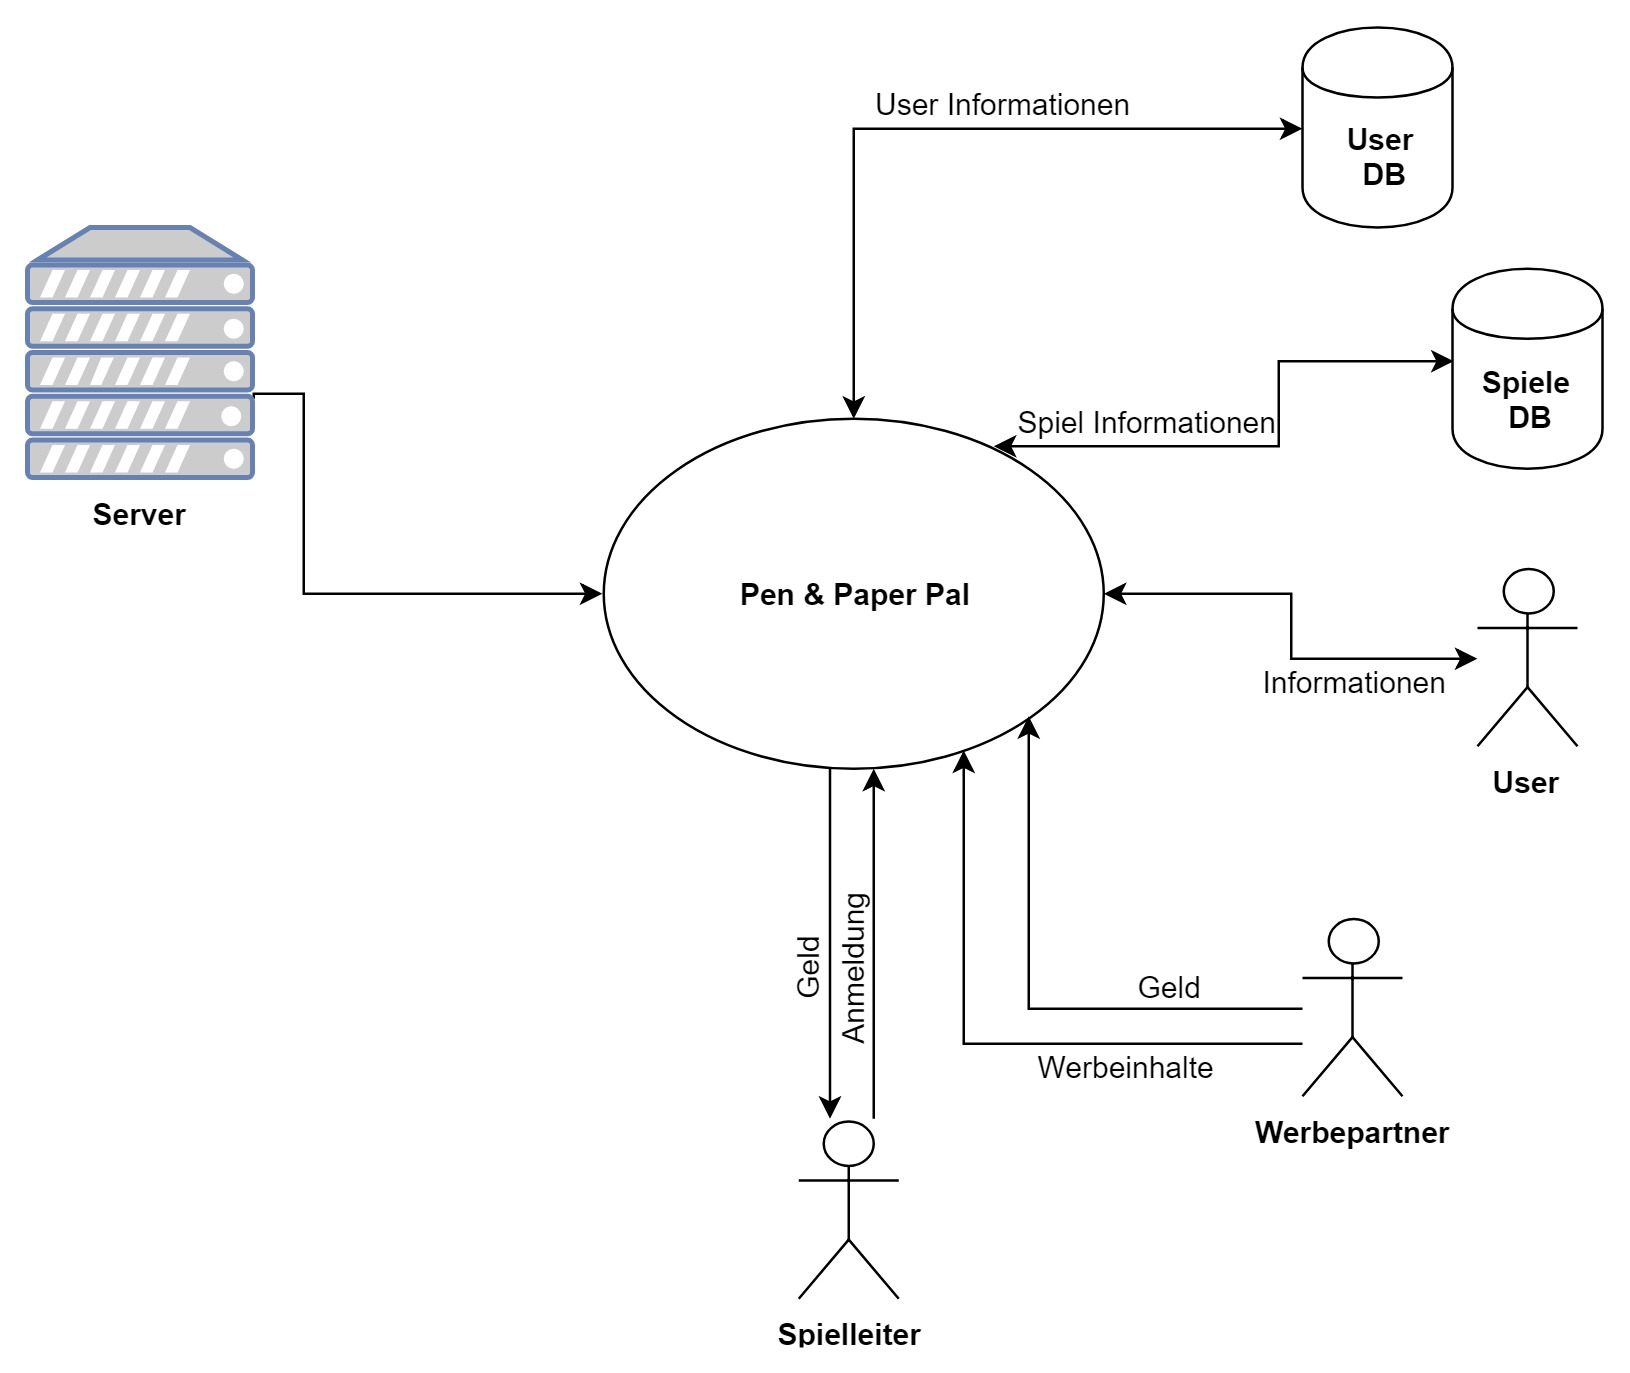
\includegraphics[width = 0.95\textwidth]{docs/0_Sonstiges/03_03_Systemkontext.jpg}
	\label{fig:SystemKontext}
 \end{figure}

\begin{landscape}
	\thispagestyle{empty}
	\newgeometry{top = 12cm,textheight=20cm,bottom = 2cm}
	\small
\section{Stakeholderanalyse}
	\begin{tabularx}{1.2\paperwidth}{|>{\cellcolor{namecolor!25}}l|l|l|X|X|X|}
		\hline
		\multicolumn{6}{|l|}{\colorcell{Stakeholderübersicht}}\\
		\hline
		\rowcolor{namecolor!25}
		Rolle&Vertreter
		\footnote{Eine detailierte Aufführung der einzelnen Personen ist in \hyperref[app:A_Personen]{Appendix A} gegeben}&Verfügbarkeit&Beschreibung &Wissennsgebiete&Begründung\\
		\hline
		Projektleitung&\hyperref[person:MarkusBauer]{Markus Bauer}&1\%& Nennt Produkt-\&Projektziele&Kennt Produkte der Konkurrenz&Entscheided über Realisierung, Geldgeber\\
		\hline
		Frontend&\hyperref[person:MariusTuschl]{Marius Tuschl}&100\%&Planung der Architektur des Frontends& Kennntnis über Framework &Entscheidung über die Realisierung des Frontends\\
		\hline
		Backend&\hyperref[person:RichardTscharntke]{Richard Tscharntke}&100\%&Planung und Architektur des Backends&Kenntnis über Framework, Monetaresierung&Entscheided über die Realisierunng des Backends\\
		\hline
		Marketing&\hyperref[person:PatrickGruber]{Patrick Gruber}&35\%&Planung Marketinngkonzept, Korrespondenz mit Werbepartner&Kennntnisse über Produktmarkt&Entscheided über die Realisierung des Marketingkonzepts\\
		\hline
		Anwender&\hyperref[person:PiaEichinger]{Pia Eichinger}&2\%&Benutzer des Systems&Erfahrene Spielerin&Bewertung des Systems aus der Sicht des Endanwenders\\
		\hline
		Gamemaster&\hyperref[person:FlorianLoher]{Florian Loher}&23\%&Erweiterter Nutzer des Systems&Langjährige Spielerfahrunng&Bewertung des Systems aus sicht des erweiterten Endanwenders\\
		\hline
		Forenadmin&\hyperref[person:FlorianLink]{Florian Link}&&&&\\
		\hline
		Zahlungsdienst&\hyperref[person:MrPayPal]{Mr. PayPal}&95\%&Wickelt Zahlungstrannsfer ab&Technische Abweicklung des Zahlunngsprozesses&International anerkanntes online Zahlungssystem\\
		\hline
		Appstore&\hyperref[person:MrGoogle]{Mr. Google}&95\%&Vertrieb der Applikation&Technische Abwicklung des Appvertriebs&Wird zum Angebot von Android Apps benötigt\\
		\hline
\end{tabularx}
\restoregeometry
\end{landscape}

\section{Umfang des Projekts}
	\subsection*{Aktueller Zustand}
	Es gibt viele Menschen, die von Pen\&Paper Spielen gehört haben und diese ausprobieren wollen. Das ist im Moment aber gar nicht so einfach. Man braucht eine Gruppe an Mitspielern, einen Spielführer und Regelwerke. Wenn man niemanden kennt, der bereits Erfahrungen mit Pen\&Paper Spielen hat, können diese Hürden unüberwindbar scheinen.\\
	Auch für erfahrene Spieler kann es schwierig sein, neue Gruppen bzw. Gruppen für andere Spiele zu finden. 	
	\subsection*{Umfang des Produktes}
	Unsere Applikation löst das beschriebene Problem durch das Zusammenbringen von begeisterten Pen\&Paper Spielern in einer intuitiven, modernen Umgebung. Pen\&Paper Freunde können sich zu Spielgruppen zusammenschließen und mithilfe unserer Anwendung auf schnelle Art und Weise neue und erfahrenere Spielpartner finden.\\
	Um das Zusammenleben der Spieler untereinander möglichst reibungslos zu gestalten ist ein Bewertungssystem für Spiele, Spieler, Spielleiter und Orte geplant. So kann der Benutzer durch einen kurzen Blick erahnen, ob für ihn eine Spielgruppe mit diesem Mensch in Frage kommt.\\
	Neben unseren Plänen für das Zusammenbringen von Spielern haben wir weiterhin vor eine Tauschbörse für Spiele anzubieten. Dadurch können Benutzer untereinander aufregende neue Spiele austauschen und kennen lernen.
	
\section{Requirementsengineering}
\begin{tabularx}{\textwidth}{|c|X|}
	\hline
	\multicolumn{2}{|l|}{\colorcell{{Functional Requirements}}}\\
	\hline
	\colorcelllight{REQ01} & Der Benutzer muss sich anmelden können.\\
	\hline
	\colorcelllight{REQ02} & Ein neuer Anwender ohne Account muss sich registrieren können.\\
	\hline
	\colorcelllight{REQ03} & Benutzer muss Orte, andere Nutzer und Spiele bewerten können.\\
	\hline
	\colorcelllight{REQ04} & Benutzer können Spielgruppen erstellen.\\
	\hline
	\colorcelllight{REQ05} & Benutzer müssen andere suchende Spieler (unter Angabe eines Ortes sowie eines Umkreises) finden können.\\
	\hline
	\colorcelllight{REQ06} & Benutzer sollen sich innerhalb der Gruppe unterhalten können.\\
	\hline
	\colorcelllight{REQ07} & Benutzer sollen untereinander kommunizieren können.\\
	\hline
	\colorcelllight{REQ08} & Benutzer soll per GPS suchende Spieler im Umkreis finden können.\\
	\hline
	\colorcelllight{REQ09} & Benutzer soll Suche filtern können.\\
	\hline
	\colorcelllight{REQ10} & Benutzer soll innerhalb der Gruppe einen gemeinsamen Termin finden können.\\
	\hline
	\colorcelllight{REQ11} & Benutzer sollen an einer Tauschbörse ihre Spiele tauschen können.\\
	\hline
	\colorcelllight{REQ12} & Benutzer sollen sich in einem Forum austauschen können.\\
	\hline
	\colorcelllight{REQ13} & Benutzer muss eigenes Profil individualisieren könne.\\
	\hline
	\colorcelllight{REQ14} & Benutzer soll Gruppen verlassen können.\\
	\multicolumn{2}{|l|}{\colorcell{Non-Functional Requirements}}\\
	\hline
	\colorcelllight{REQ15} & Server muss immer erreichbar sein.\\
	\hline
	\colorcelllight{REQ16} & Server muss durchschnittlich innerhalb von 20ms antworten.\\
	\hline
	\colorcelllight{REQ17} & Miner muss immer minen.\\
	\hline
	\colorcelllight{REQ18} & Das Projekt soll nach Kanban geführt werden.\\
	\hline
	\multicolumn{2}{|l|}{\colorcell{Risiken}}\\
	\hline
	\colorcelllight{RSK01} & Größe des Projekts wurde überschätzt (Projekt \& Produkt).\\
	\hline
	\colorcelllight{RSK02} & Ein Konkurrenz-Produkt erreicht den Markt vor Systemfertigstellung.\\
	\hline
	\colorcelllight{RSK03} & Projekt erwirtschaftet zu wenig Geld.\\
	\hline
\end{tabularx}

\section{Kano-Modell}
\begin{tabularx}{\textwidth}{|>{\colorcelllight{}}l|l|X|X|l|l|}
	\colorcell{REQ}&\colorcell{Kategorie}&\colorcell{Zufriedenheit}&\colorcell{Erfüllungsgrad}&\colorcell{$\frac{\text{Aufwand}}{\text{Nutzen}}$}&\colorcell{Prioritär}\\
	\hline
	\colorcelllight{01}&Basis&0&100\%&\textcolor{green}{$\Uparrow$}&1\\
	\hline
	02&Basis&0&100\%&\textcolor{green}{$\Uparrow$}&1\\
	\hline
	03&Basis&0&100\%&\textcolor{green}{$\Uparrow$}&1\\
	\hline
	04&Basis&0&100\%&\textcolor{green}{$\Uparrow$}&1\\
	\hline
	05&Basis&0&100\%&\textcolor{green}{$\Uparrow$}&1\\
	\hline
	06&Leistung&0&50\%&\textcolor{orange}{$\Rightarrow$}&2\\
	\hline
	07&Leistung&0.3&60\%&\textcolor{orange}{$\Rightarrow$}&2\\
	\hline
	08&Begeisterung&0.1&25\%&\textcolor{orange}{$\Rightarrow$}&3\\
	\hline
	09&Leistung&0.8&80\%&\textcolor{orange}{$\Rightarrow$}&2\\
	\hline
	10&Begeisterung&0.25&40\%&\textcolor{green}{$\Uparrow$}&2\\
	\hline
	11&Begeisterung&0.2&33\%&\textcolor{orange}{$\Rightarrow$} /\textcolor{red}{$\Downarrow$}&3\\
	\hline
	12&Begeisterung&0.2&33\%&\textcolor{red}{$\Downarrow$}&3\\
	\hline
	13&Basis&0&100\%&\textcolor{green}{$\Uparrow$}&1\\
	\hline
	14&Basis&0&100\%&\textcolor{green}{$\Uparrow$}&1\\
	\hline
\end{tabularx}

\newpage
\begin{landscape}
	\thispagestyle{empty}
	\newgeometry{left = 1.5cm,top = 11cm,textheight=25cm}
	\section{UseCase Diagram}
	\begin{figure}[h!]
		\centering
		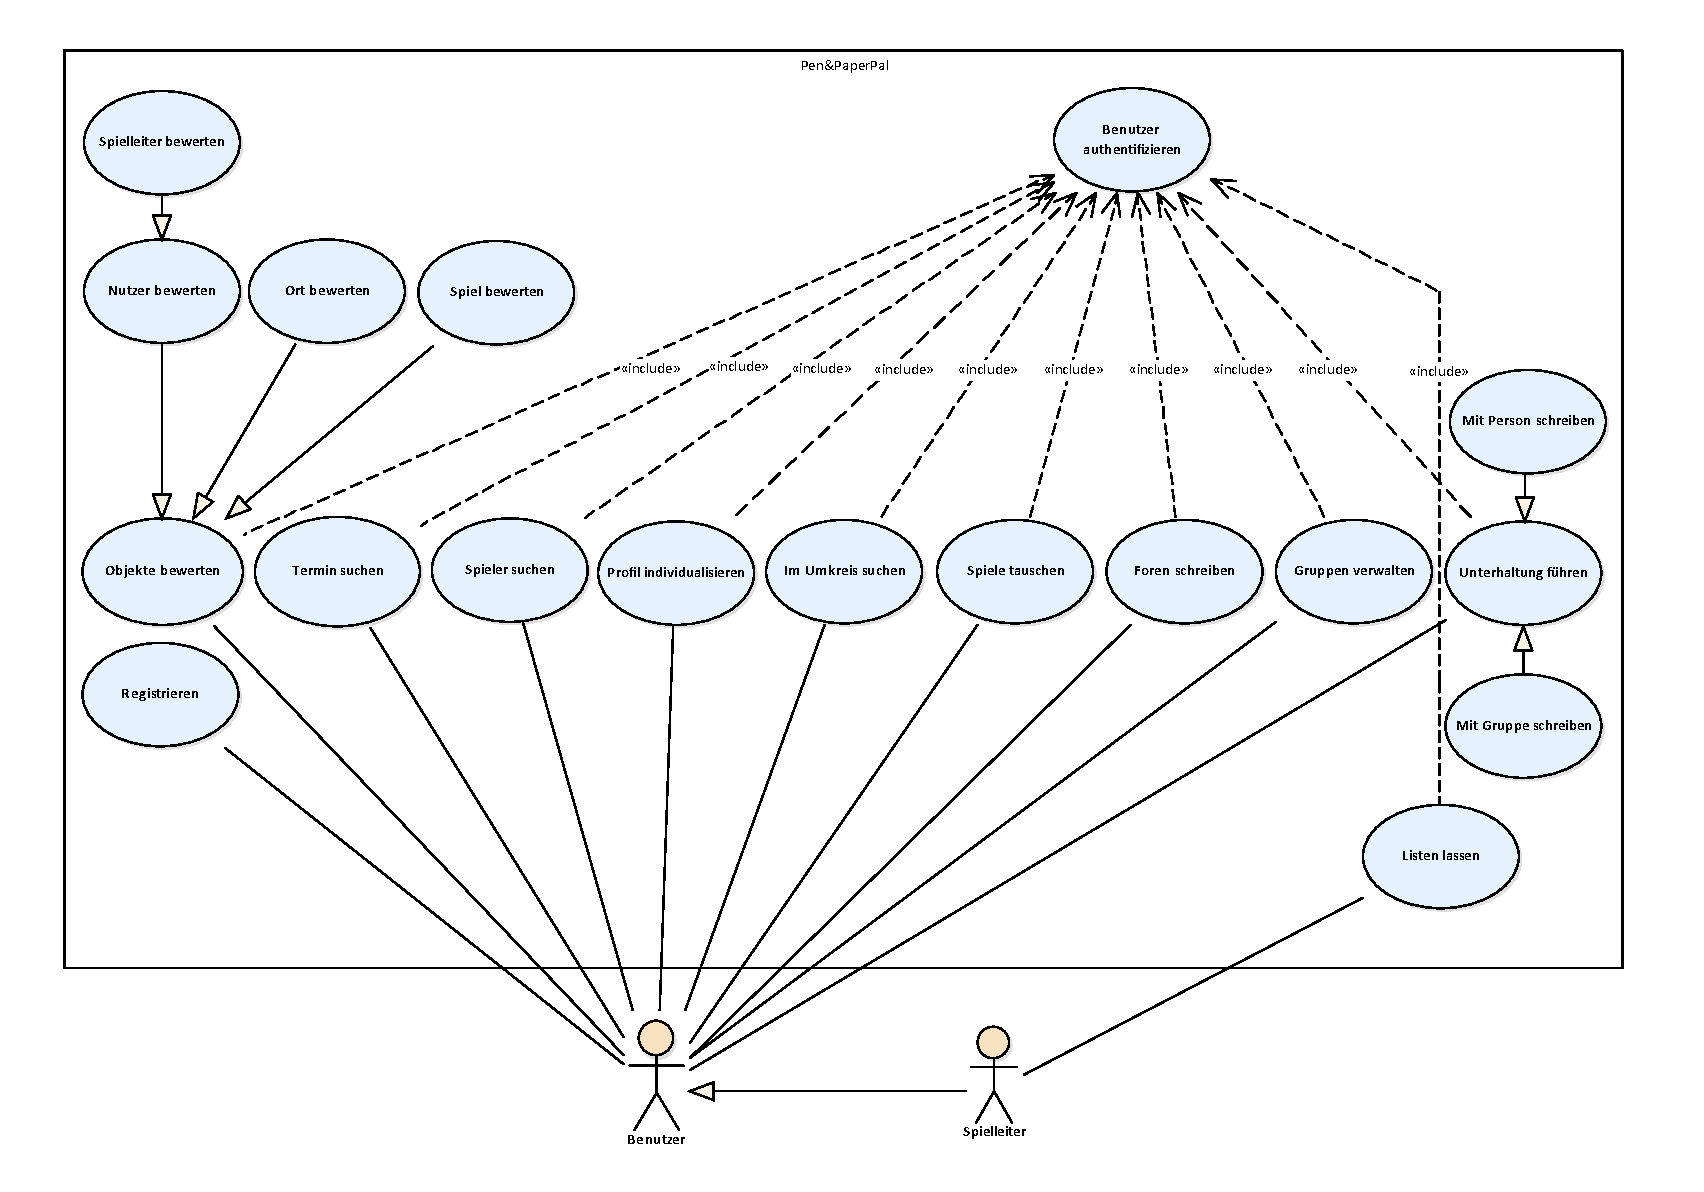
\includegraphics[width=\textheight]{docs/1_UseCaseDiagramme/PrimaryUseCases.pdf}
		\label{fig:UCD}
	\end{figure}
	\restoregeometry
\end{landscape}

\newpage
\section{UseCase Beschreibungen}
\newlength\xlength
\settowidth\xlength{Alternativszenarien}
\addtolength\xlength{4\tabcolsep}

\newlength\ylength
\setlength\ylength\mylength
\addtolength\ylength{-\xlength}

\subsection*{Profil Individualisieren}
\label{tab:UCB_ProfilIndividualisieren}
\begin{tabularx}{\textwidth}{|>{\colorcelllight{}}l|X|X|X|X|}
	\hline
	\multicolumn{5}{|l|}{\colorcell{Use-Case Beschreibung}}\\
	\hline
	Name&\multicolumn{4}{p{\ylength}|}{Profil individualisieren}\\
	\hline
	Kurzbeschreibung&\multicolumn{4}{p{\ylength}|}{Benutzer kann Gesichtspunkte seines Profils gestalten.}\\
	\hline
	Akteure&\multicolumn{4}{p{\ylength}|}{Benutzer}\\
	\hline
	Auslöser&\multicolumn{4}{p{\ylength}|}{Benutzer}\\
	\hline
	Eingehende Daten&\multicolumn{4}{p{\ylength}|}{Name, Geburtsdatum, Wohnort, Spielliste, Biographie}\\
	\hline
	Vorbedingungen&\multicolumn{4}{p{\ylength}|}{Benutzer authentifiziert}\\
	\hline
	Nachbedingungen&\multicolumn{4}{p{\ylength}|}{Aktualisiertes Nutzerprofil}\\
	\hline
	Essentielle Schritte&\multicolumn{4}{p{\ylength}|}{
	1. Benutzer authentifizieren.
	\newline
	2. Benutzer gibt zu erneuernde Profildaten ein.
	\newline
	3. Benutzerprofil aktualisieren.
	}\\
	\hline
	Alternativszenarien&\multicolumn{4}{p{\ylength}|}{
	Nutzer gibt fehlerhafte Daten ein.
	\newline
	1. Fehlermeldung anzeigen.
	\newline
	2. Nutzer zur erneuten Eingabe auffordern.
	}\\
	\hline
	Offene Punkte&\multicolumn{4}{p{\ylength}|}{}\\
	\hline
	Änderungshistorie&{\footnotesize\underline{\texttt{Wann}}}&{\footnotesize\underline{\texttt{Wer}}}&{\footnotesize\underline{\texttt{Neuer Status}}}&{\footnotesize\underline{\texttt{Was}}}\\
	&15.05.18&\hyperref[person:PatrickGruber]{Patrick Gruber}&Fertig&Erstellung\\
	\hline
	Sonstiges&\multicolumn{4}{p{\ylength}|}{}\\
	\hline
	Ersteller&\multicolumn{4}{p{\ylength}|}{\hyperref[person:PatrickGruber]{Patrick Gruber}}\\
	\hline
\end{tabularx}

\subsection*{Foreneintrag Schreiben}
\label{tab:UCB_ForeneintragSchreiben}
\begin{tabularx}{\textwidth}{|>{\colorcelllight{}}l|X|X|X|X|}
	\hline
	\multicolumn{5}{|l|}{\colorcell{Use-Case Beschreibung}}\\
	\hline
	Name&\multicolumn{4}{p{\ylength}|}{Foreneintrag schreiben}\\
	\hline
	Kurzbeschreibung&\multicolumn{4}{p{\ylength}|}{Benutzer kann einen Eintrag im Forum verfassen und posten}\\
	\hline
	Akteure&\multicolumn{4}{p{\ylength}|}{Benutzer, Forenadmin}\\
	\hline
	Auslöser&\multicolumn{4}{p{\ylength}|}{Benutzer, Forenadmin}\\
	\hline
	Eingehende Daten&\multicolumn{4}{p{\ylength}|}{Text, den der Benutzer als Eintrag im Forum posten möchte}\\
	\hline
	Vorbedingungen&\multicolumn{4}{p{\ylength}|}{Benutzer authentifiziert}\\
	\hline
	Nachbedingungen&\multicolumn{4}{p{\ylength}|}{Foreneintrag erstellt und im Forum dargestellt}\\
	\hline
	Essentielle Schritte&\multicolumn{4}{p{\ylength}|}{
	1. Benutzer authentifizieren.
	\newline
	2. Benutzer verfasst Text.
	\newline
	3. Eintrag wird gepostet.
	}\\
	\hline
	Alternativszenarien&\multicolumn{4}{p{\ylength}|}{
	Benutzer erstellt Kopie eines anderen Beitrags.
	\newline
	1. Fehlermeldung ausgeben, dass Eintrag bereits existiert.
	\newline
	2. Benutzer Link zu diesem Eintrag anzeigen.
	}\\
	\hline
	Offene Punkte&\multicolumn{4}{p{\ylength}|}{}\\
	\hline
	Änderungshistorie&{\footnotesize\underline{\texttt{Wann}}}&{\footnotesize\underline{\texttt{Wer}}}&{\footnotesize\underline{\texttt{Neuer Status}}}&{\footnotesize\underline{\texttt{Was}}}\\
	&15.05.18&\hyperref[person:PatrickGruber]{Patrick Gruber}&Fertig&Erstellung\\
	\hline
	Sonstiges&\multicolumn{4}{p{\ylength}|}{}\\
	\hline
	Ersteller&\multicolumn{4}{p{\ylength}|}{\hyperref[person:PatrickGruber]{Patrick Gruber}}\\
	\hline
\end{tabularx}

\subsection*{Spieler Suchen}
\label{tab:UCB_SpielerSuchen}
\begin{tabularx}{\textwidth}{|>{\colorcelllight{}}l|X|X|X|X|}
	\hline
	\multicolumn{5}{|l|}{\colorcell{UseCase Beschreibung}}\\
	\hline
	Name&\multicolumn{4}{p{\ylength}|}{Spieler suchen}\\
	\hline
	Kurzbeschreibung&\multicolumn{4}{p{\ylength}|}{Benutzer die Spielersuche zu ermöglichen}\\
	\hline
	Akteure&\multicolumn{4}{p{\ylength}|}{Benutzer, Spielleiter}\\
	\hline
	Auslöser&\multicolumn{4}{p{\ylength}|}{Benutzer/Spielleiter fehlen noch Mitspieler }\\
	\hline
	Eingehende Daten&\multicolumn{4}{p{\ylength}|}{Umkreis, Spiel, (Termin optional)}\\
	\hline
	Vorbedingungen&\multicolumn{4}{p{\ylength}|}{keine}\\
	\hline
	Nachbedingungen&\multicolumn{4}{p{\ylength}|}{Benutzer/Spielleiter bekommt Spieler anhand der eingegangenen Daten angezeigt. }\\
	\hline
	Essentielle Schritte&\multicolumn{4}{p{\ylength}|}{1. Benutzer Authentifizieren
	\newline
	2. Daten für Filterung eingeben
	\newline
	3. Benutzer aus Datenbank auswählen/anschreiben}\\
	\hline
	Alternativszenarien&\multicolumn{4}{p{\ylength}|}{Keine Spieler mit aktuellen Filtereingaben auffindbar:
	\newline
	1. Fehlermeldung anzeigen
	\newline
	Authentifizierung Fehlgeschalgen:
	\newline
	1. Fehlermeldung anzeigen}\\
	\hline
	Offene Punkte&\multicolumn{4}{p{\ylength}|}{erweiterte Filtereinstellungen}\\
	\hline
	Änderungshistorie&Wann&Wer&Neuer Status&Was\\
	&09.05.18&\hyperref[person:MarkusBauer]{Markus Bauer}&fertig&Erstellung\\
	\hline
	Sonstiges&\multicolumn{4}{p{\ylength}|}{}\\
	\hline
	Ersteller&\multicolumn{4}{p{\ylength}|}{\hyperref[person:MarkusBauer]{Markus Bauer}}\\
	\hline
\end{tabularx}

\subsection*{Termin Suchen}
\label{tab:UCB_TerminSuchen}
\begin{tabularx}{\textwidth}{|>{\colorcelllight{}}l|X|X|X|X|}
	\hline
	\multicolumn{5}{|l|}{\colorcell{UseCase Beschreibung}}\\
	\hline
	Name&\multicolumn{4}{p{\ylength}|}{Termin suchen}\\
	\hline
	Kurzbeschreibung&\multicolumn{4}{p{\ylength}|}{Benutzer/Spielleiter die Terminfindung zu ermöglichen}\\
	\hline
	Akteure&\multicolumn{4}{p{\ylength}|}{Benutzer/Spielleiter}\\
	\hline
	Auslöser&\multicolumn{4}{p{\ylength}|}{Gruppe von Spieler hat sich gefunden und sucht noch einen passenden Termin.}\\
	\hline
	Eingehende Daten&\multicolumn{4}{p{\ylength}|}{Terminvorschläge (Datum,Uhrzeit,Länge) der verschiedenen Benutzer}\\
	\hline
	Vorbedingungen&\multicolumn{4}{p{\ylength}|}{keine}\\
	\hline
	Nachbedingungen&\multicolumn{4}{p{\ylength}|}{Spieler haben einen für alle passenden Termin gefunden}\\
	\hline
	Essentielle Schritte&\multicolumn{4}{p{\ylength}|}{1. Benutzer Authentifizieren
	\newline
	2. Benutzer gibt für Ihn passende Termine ein
	\newline
	3. System zeigt passende Termine an
	\newline
	4. Benutzer einigen sich auf einen Termin}\\
	\hline
	Alternativszenarien&\multicolumn{4}{p{\ylength}|}{Authentifizierung fehlgeschalgen:
	\newline
	1. Fehlermeldung anzeigen
	\newline
	Keinen übereinstimmenden Termin gefunden:
	\newline
	1. Meldung an die Spieler}\\
	\hline
	Offene Punkte&\multicolumn{4}{p{\ylength}|}{}\\
	\hline
	Änderungshistorie&Wann&Wer&Neuer Status&Was\\
	&09.05.18&\hyperref[person:MarkusBauer]{Markus Bauer}&Fertig&Erstellung\\
	\hline
	Sonstiges&\multicolumn{4}{p{\ylength}|}{}\\
	\hline
	Ersteller&\multicolumn{4}{p{\ylength}|}{\hyperref[person:MarkusBauer]{Markus Bauer}}\\
	\hline
\end{tabularx}
\subsection*{Blahh}
\label{tab:UCB}
\begin{tabularx}{\textwidth}{|>{\colorcelllight{}}l|X|X|X|X|}
	\hline
	\multicolumn{5}{|l|}{\colorcell{UseCase Beschreibung}}\\
	\hline
	Name&\multicolumn{4}{p{\ylength}|}{Marius Kann Latex richtig!!}\\
	\hline
	Kurzbeschreibung&\multicolumn{4}{p{\ylength}|}{}\\
	\hline
	Akteure&\multicolumn{4}{p{\ylength}|}{}\\
	\hline
	Auslöser&\multicolumn{4}{p{\ylength}|}{}\\
	\hline
	Eingehende Daten&\multicolumn{4}{p{\ylength}|}{}\\
	\hline
	Vorbedingungen&\multicolumn{4}{p{\ylength}|}{}\\
	\hline
	Nachbedingungen&\multicolumn{4}{p{\ylength}|}{}\\
	\hline
	Essentielle Schritte&\multicolumn{4}{p{\ylength}|}{}\\
	\hline
	Alternativszenarien&\multicolumn{4}{p{\ylength}|}{}\\
	\hline
	Offene Punkte&\multicolumn{4}{p{\ylength}|}{}\\
	\hline
	Änderungshistorie&Wann&Wer&Neuer Status&Was\\
	&Bald&Nicht Ich&Fertig&DeineMutter!\\
	\hline
	Sonstiges&\multicolumn{4}{p{\ylength}|}{}\\
	\hline
	Ersteller&\multicolumn{4}{p{\ylength}|}{\hyperref[person:MariusTuschl]{Marius Tuschl}}\\
	\hline
\end{tabularx}
\vfill
\subsection*{Bluhh}
\label{tab:UCB}
\begin{tabularx}{\textwidth}{|>{\colorcelllight{}}l|X|X|X|X|}
	\hline
	\multicolumn{5}{|l|}{\colorcell{UseCase Beschreibung}}\\
	\hline
	Name&\multicolumn{4}{p{\ylength}|}{Marius Kann Latex richtig!!}\\
	\hline
	Kurzbeschreibung&\multicolumn{4}{p{\ylength}|}{}\\
	\hline
	Akteure&\multicolumn{4}{p{\ylength}|}{}\\
	\hline
	Auslöser&\multicolumn{4}{p{\ylength}|}{}\\
	\hline
	Eingehende Daten&\multicolumn{4}{p{\ylength}|}{}\\
	\hline
	Vorbedingungen&\multicolumn{4}{p{\ylength}|}{}\\
	\hline
	Nachbedingungen&\multicolumn{4}{p{\ylength}|}{}\\
	\hline
	Essentielle Schritte&\multicolumn{4}{p{\ylength}|}{}\\
	\hline
	Alternativszenarien&\multicolumn{4}{p{\ylength}|}{}\\
	\hline
	Offene Punkte&\multicolumn{4}{p{\ylength}|}{}\\
	\hline
	Änderungshistorie&Wann&Wer&Neuer Status&Was\\
	&Bald&Nicht Ich&Fertig&DeineMutter!\\
	\hline
	Sonstiges&\multicolumn{4}{p{\ylength}|}{}\\
	\hline
	Ersteller&\multicolumn{4}{p{\ylength}|}{\hyperref[person:MariusTuschl]{Marius Tuschl}}\\
	\hline
\end{tabularx}

\subsection*{Bewerten}
\label{tab:UCB}
\begin{tabularx}{\textwidth}{|>{\colorcelllight{}}l|X|X|X|X|}
	\hline
	\multicolumn{5}{|l|}{\colorcell{UseCase Beschreibung}}\\
	\hline
	Name&\multicolumn{4}{p{\ylength}|}{Bewerten}\\
	\hline
	Kurzbeschreibung&\multicolumn{4}{p{\ylength}|}{Bewertung von Spiel, Spielleiter, Gruppe oder Location}\\
	\hline
	Akteure&\multicolumn{4}{p{\ylength}|}{Benutzer}\\
	\hline
	Auslöser&\multicolumn{4}{p{\ylength}|}{Der Benutzer möchte etwas bewerten}\\
	\hline
	Eingehende Daten&\multicolumn{4}{p{\ylength}|}{Bewertung, Thema}\\
	\hline
	Vorbedingungen&\multicolumn{4}{p{\ylength}|}{Angemeldet}\\
	\hline
	Nachbedingungen&\multicolumn{4}{p{\ylength}|}{Bewertung wird erstellt}\\
	\hline
	Essentielle Schritte&\multicolumn{4}{p{\ylength}|}{1.  Prüfen, dass der Benutzer die Bewertung abgeben darf.\newline
	2. Bewertung wird erstellt\newline
	3. Bewertung abspeichern}\\
	\hline
	Alternativszenarien&\multicolumn{4}{p{\ylength}|}{- 	Keine Berechtigung\newline
- Keine Änderungen}\\
	\hline
	Offene Punkte&\multicolumn{4}{p{\ylength}|}{-keine-}\\
	\hline
	Änderungshistorie&{\footnotesize\underline{\texttt{Wann}}}&{\footnotesize\underline{\texttt{Wer}}}&{\footnotesize\underline{\texttt{Neuer Status}}}&{\footnotesize\underline{\texttt{Was}}}\\
	&30.05.2018&RT&FUCKING DONE BOIS&Neu erstellt!\\
	\hline
	Sonstiges&\multicolumn{4}{p{\ylength}|}{}\\
	\hline
	Ersteller&\multicolumn{4}{p{\ylength}|}{\hyperref[person:RichardTscharntke]{Richard Tscharntke}}\\
	\hline
\end{tabularx}
\vfill
\subsection*{Gruppe verwalten}
\label{tab:UCB}
\begin{tabularx}{\textwidth}{|>{\colorcelllight{}}l|X|X|X|X|}
	\hline
	\multicolumn{5}{|l|}{\colorcell{UseCase Beschreibung}}\\
	\hline
	Name&\multicolumn{4}{p{\ylength}|}{Gruppe verwalten}\\
	\hline
	Kurzbeschreibung&\multicolumn{4}{p{\ylength}|}{Verwalten oder Verlassen einer Gruppe}\\
	\hline
	Akteure&\multicolumn{4}{p{\ylength}|}{Benutzer / Spielleiter}\\
	\hline
	Auslöser&\multicolumn{4}{p{\ylength}|}{Eine Änderung an der Gruppe soll durchgeführt werden.}\\
	\hline
	Eingehende Daten&\multicolumn{4}{p{\ylength}|}{Gruppe}\\
	\hline
	Vorbedingungen&\multicolumn{4}{p{\ylength}|}{Angemeldet}\\
	\hline
	Nachbedingungen&\multicolumn{4}{p{\ylength}|}{Änderungen an der Gruppe werden gespeichert}\\
	\hline
	Essentielle Schritte&\multicolumn{4}{p{\ylength}|}{1. <<include>>: Berechtigung prüfen\newline
2. Gruppendaten anzeigen\newline
3. Änderungen erfassen\newline
4. Geänderte Gruppendaten in der Datenbank ablegen
}\\
	\hline
	Alternativszenarien&\multicolumn{4}{p{\ylength}|}{-	Keine Berechtigung\newline
-	Keine Änderungen
}\\
	\hline
	Offene Punkte&\multicolumn{4}{p{\ylength}|}{-Keine-}\\
	\hline
	Änderungshistorie&{\footnotesize\underline{\texttt{Wann}}}&{\footnotesize\underline{\texttt{Wer}}}&{\footnotesize\underline{\texttt{Neuer Status}}}&{\footnotesize\underline{\texttt{Was}}}\\
	&16.05.2018&RT&FUCKING DONE BOIS&Neu erstellt!\\
	\hline
	Sonstiges&\multicolumn{4}{p{\ylength}|}{Die einzige Möglichkeit für den Benutzer eine Änderung an der Gruppe vorzunehmen ist auszutreten.}\\
	\hline
	Ersteller&\multicolumn{4}{p{\ylength}|}{\hyperref[person:RichardTscharntke]{Richard Tscharntke}}\\
	\hline
\end{tabularx}


\pagebreak
\section{Aktivtitätsdiagramme}
\vfill

\subsection*{Profil Individualisieren}

\begin{figure}[h]
	\centering
	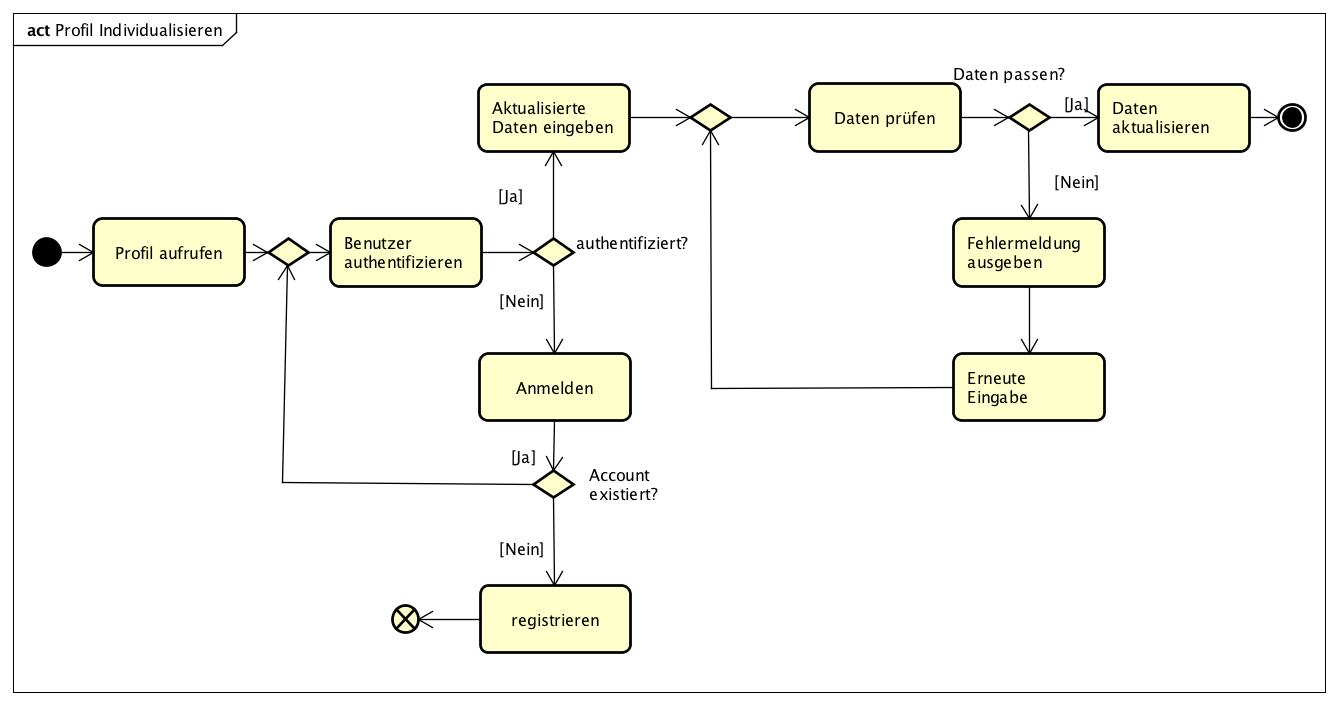
\includegraphics[width=0.8\linewidth]{docs/3_Aktivitaetsdiagramme/Patrick/Profil_Individualisieren.png}
	\label{fig:ActDia_Profil_Individualisieren}
\end{figure}

\vfill

\subsection*{Foreneintrag Schreiben}
\begin{figure}[h]
	\centering
	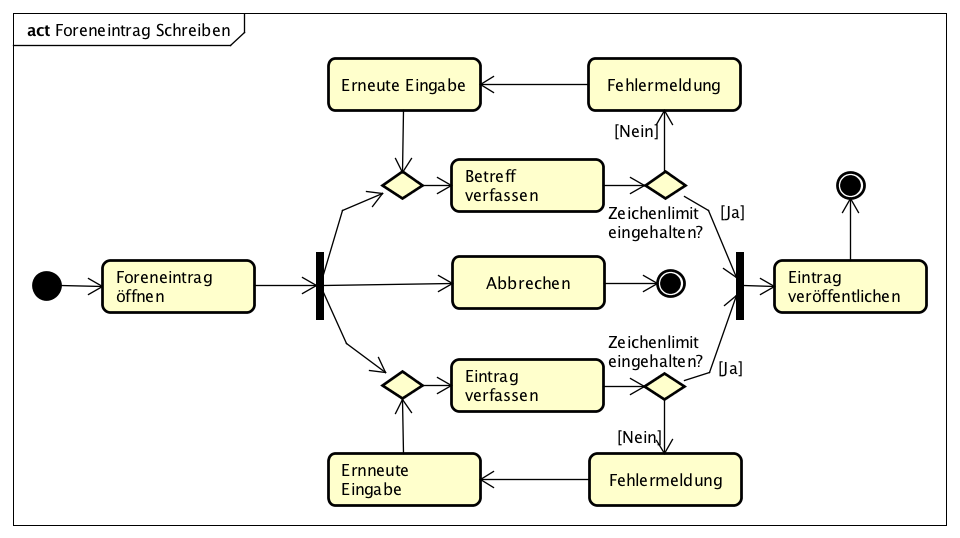
\includegraphics[width=0.8\linewidth]{docs/3_Aktivitaetsdiagramme/Patrick/Foreneintrag_Schreiben.png}
	\label{fig:ActDia_Foreneinntrag_Schreiben}
\end{figure}
\vfill

\pagebreak

\vfill

\subsection*{Forum Verwalten}
\begin{figure}[h]
	\centering
	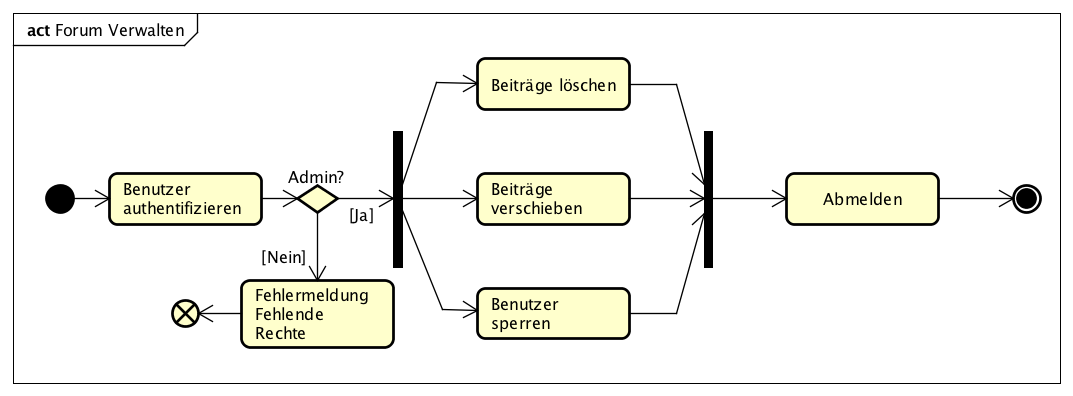
\includegraphics[width=0.8\linewidth]{docs/3_Aktivitaetsdiagramme/Patrick/Forum_Verwalten.png}
	\label{fig:ActDia_Forum_Verwalten}
\end{figure}

\vfill

\subsection*{Spiel Tauschen}
\begin{figure}[h]
	\centering
	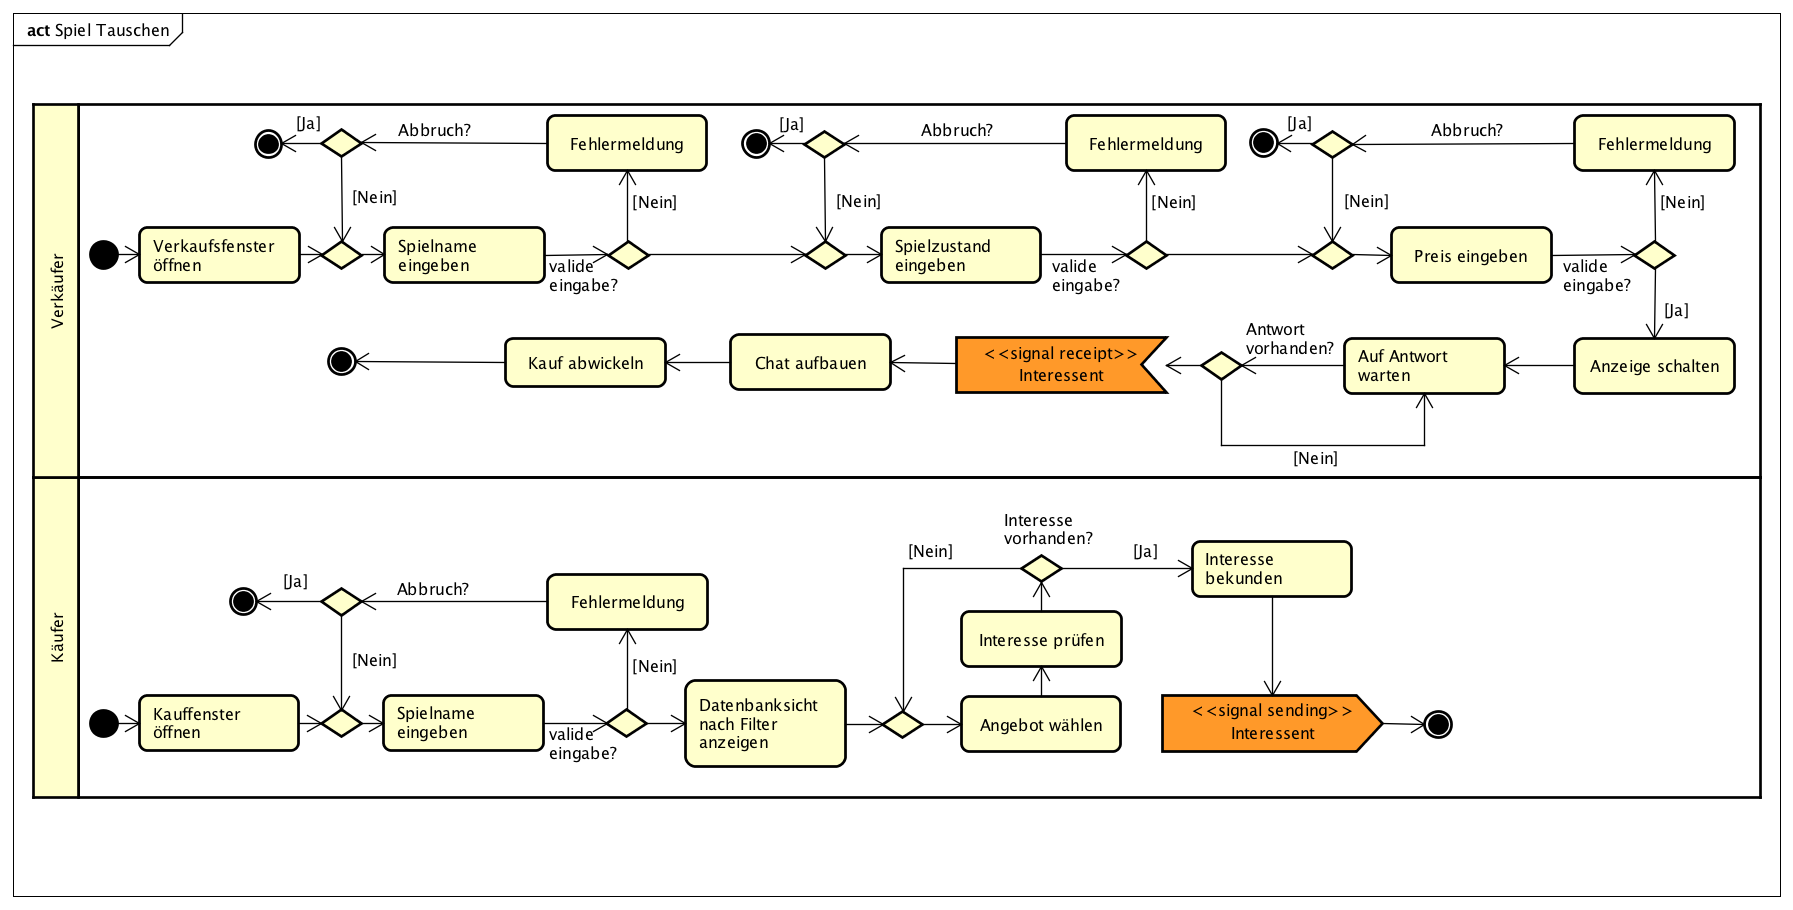
\includegraphics[width=\linewidth]{docs/3_Aktivitaetsdiagramme/Patrick/Spiel_Tauschen.png}
	\label{fig:ActDia_Spiel_Tauschen}
\end{figure}

\vfill
\pagebreak

\vfill

\subsection*{Listen Lassen}
\begin{figure}[h!]
	\centering
	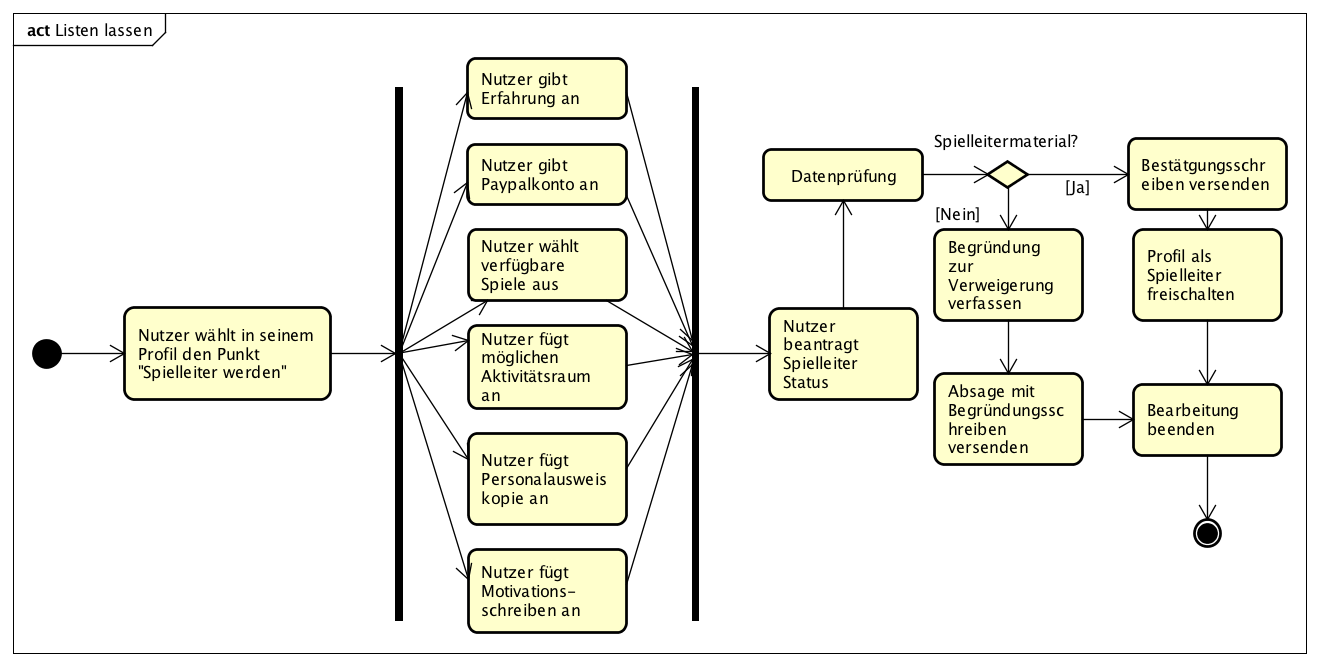
\includegraphics[width=0.8\linewidth]{docs/3_Aktivitaetsdiagramme/Markus/Listen_Lassen.png}
	\label{fig:ActDia_Listen_Lassen}
\end{figure}

\vfill

\pagebreak

\vfill

\subsection*{Spieler Suchen}
\begin{figure}[h!]
	\centering
	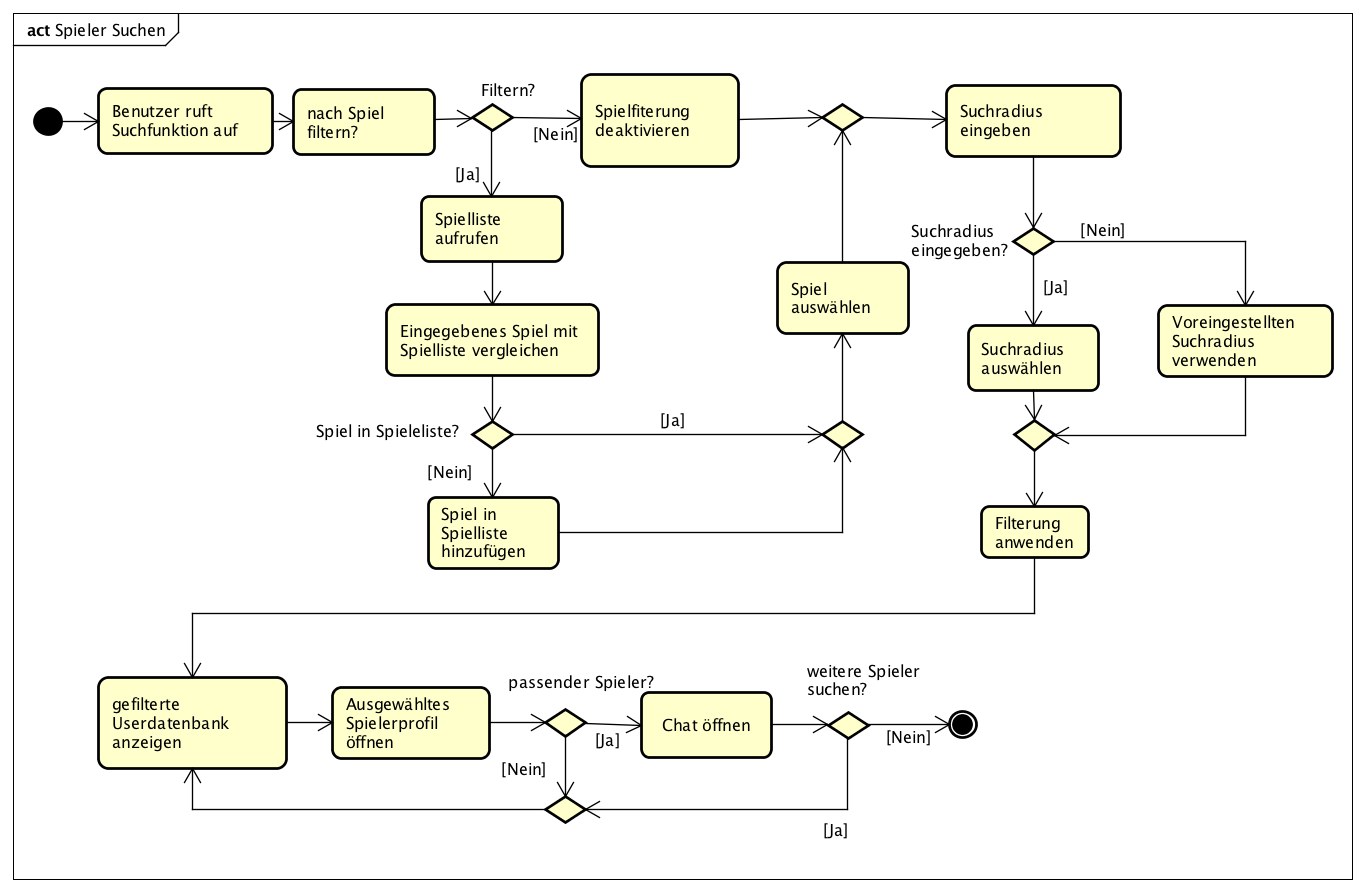
\includegraphics[width=0.8\linewidth]{docs/3_Aktivitaetsdiagramme/Markus/Spieler_Suchen.png}
	\label{fig:ActDia_Spieler_Suchen}
\end{figure}

\vfill

\subsection*{Termin Suchen}
\begin{figure}[h!]
	\centering
%	\includegraphics[width=0.8\linewidth]{}
	\label{fig:ActDia_Termin_Suchen}
\end{figure}

\vfill

\pagebreak
\vfill

\subsection*{Anmelden}
\begin{figure}[h!]
	\centering
	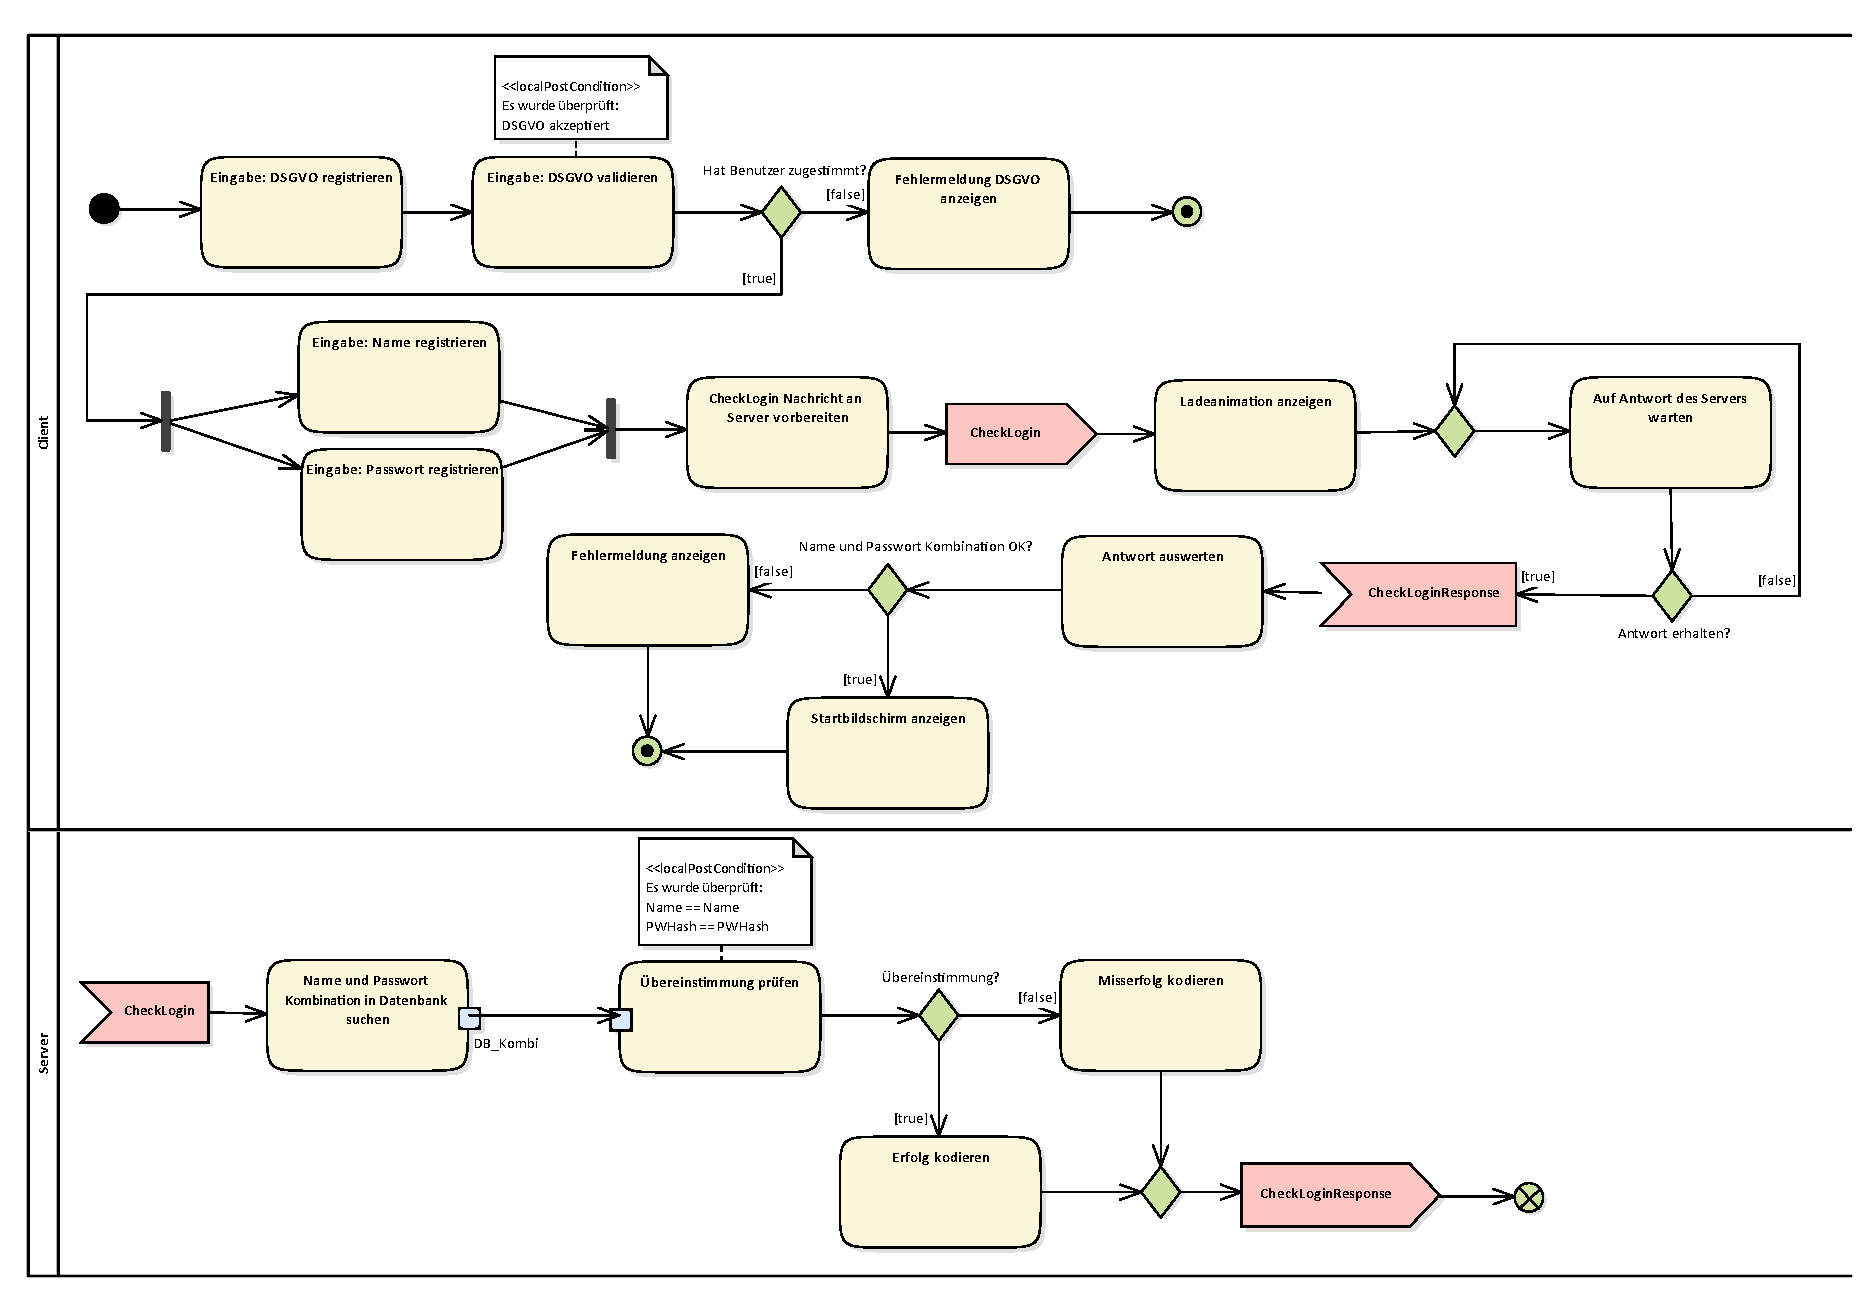
\includegraphics[width=0.9\linewidth]{docs/3_Aktivitaetsdiagramme/Marius/Anmelden.pdf}
	\label{fig:ActDia_Anmelden}
\end{figure}

\vfill

\subsection*{Registrieren}
\begin{figure}[h!]
	\centering
	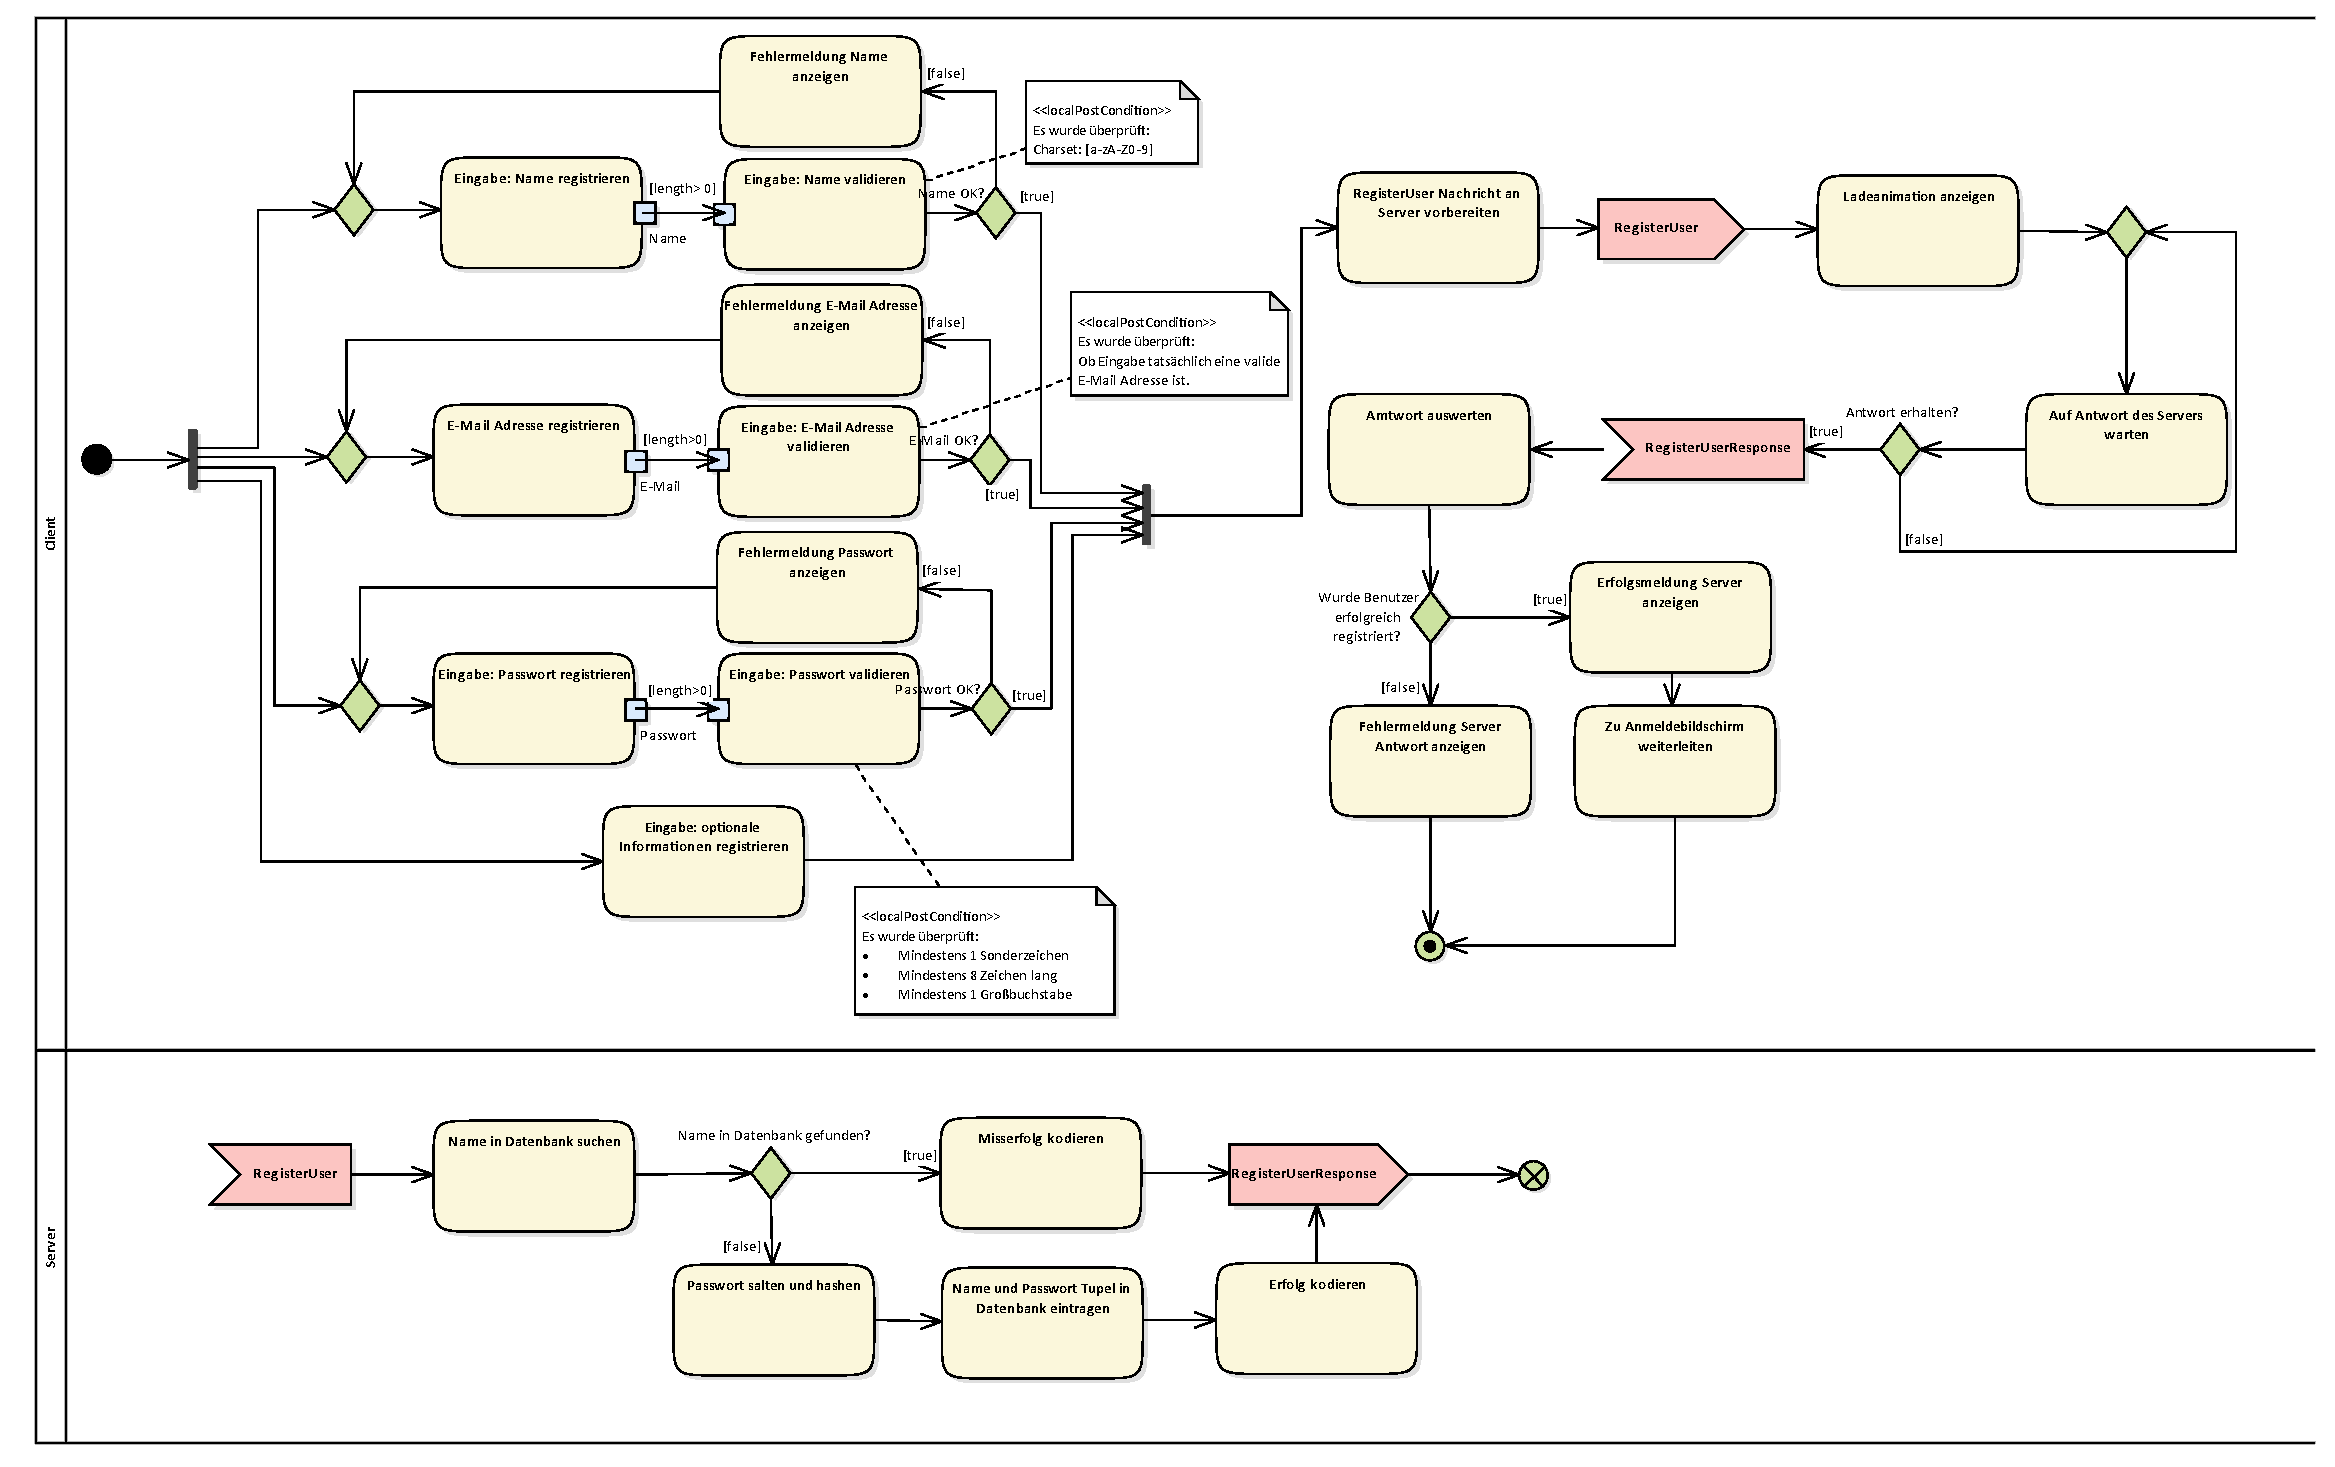
\includegraphics[width=0.9\linewidth]{docs/3_Aktivitaetsdiagramme/Marius/Registrieren.pdf}
	\label{fig:ActDia_Registrieren}
\end{figure}

\vfill
\pagebreak
\vfill

\subsection*{Gruppe Erstellen}
\begin{figure}[h!]
	\centering
	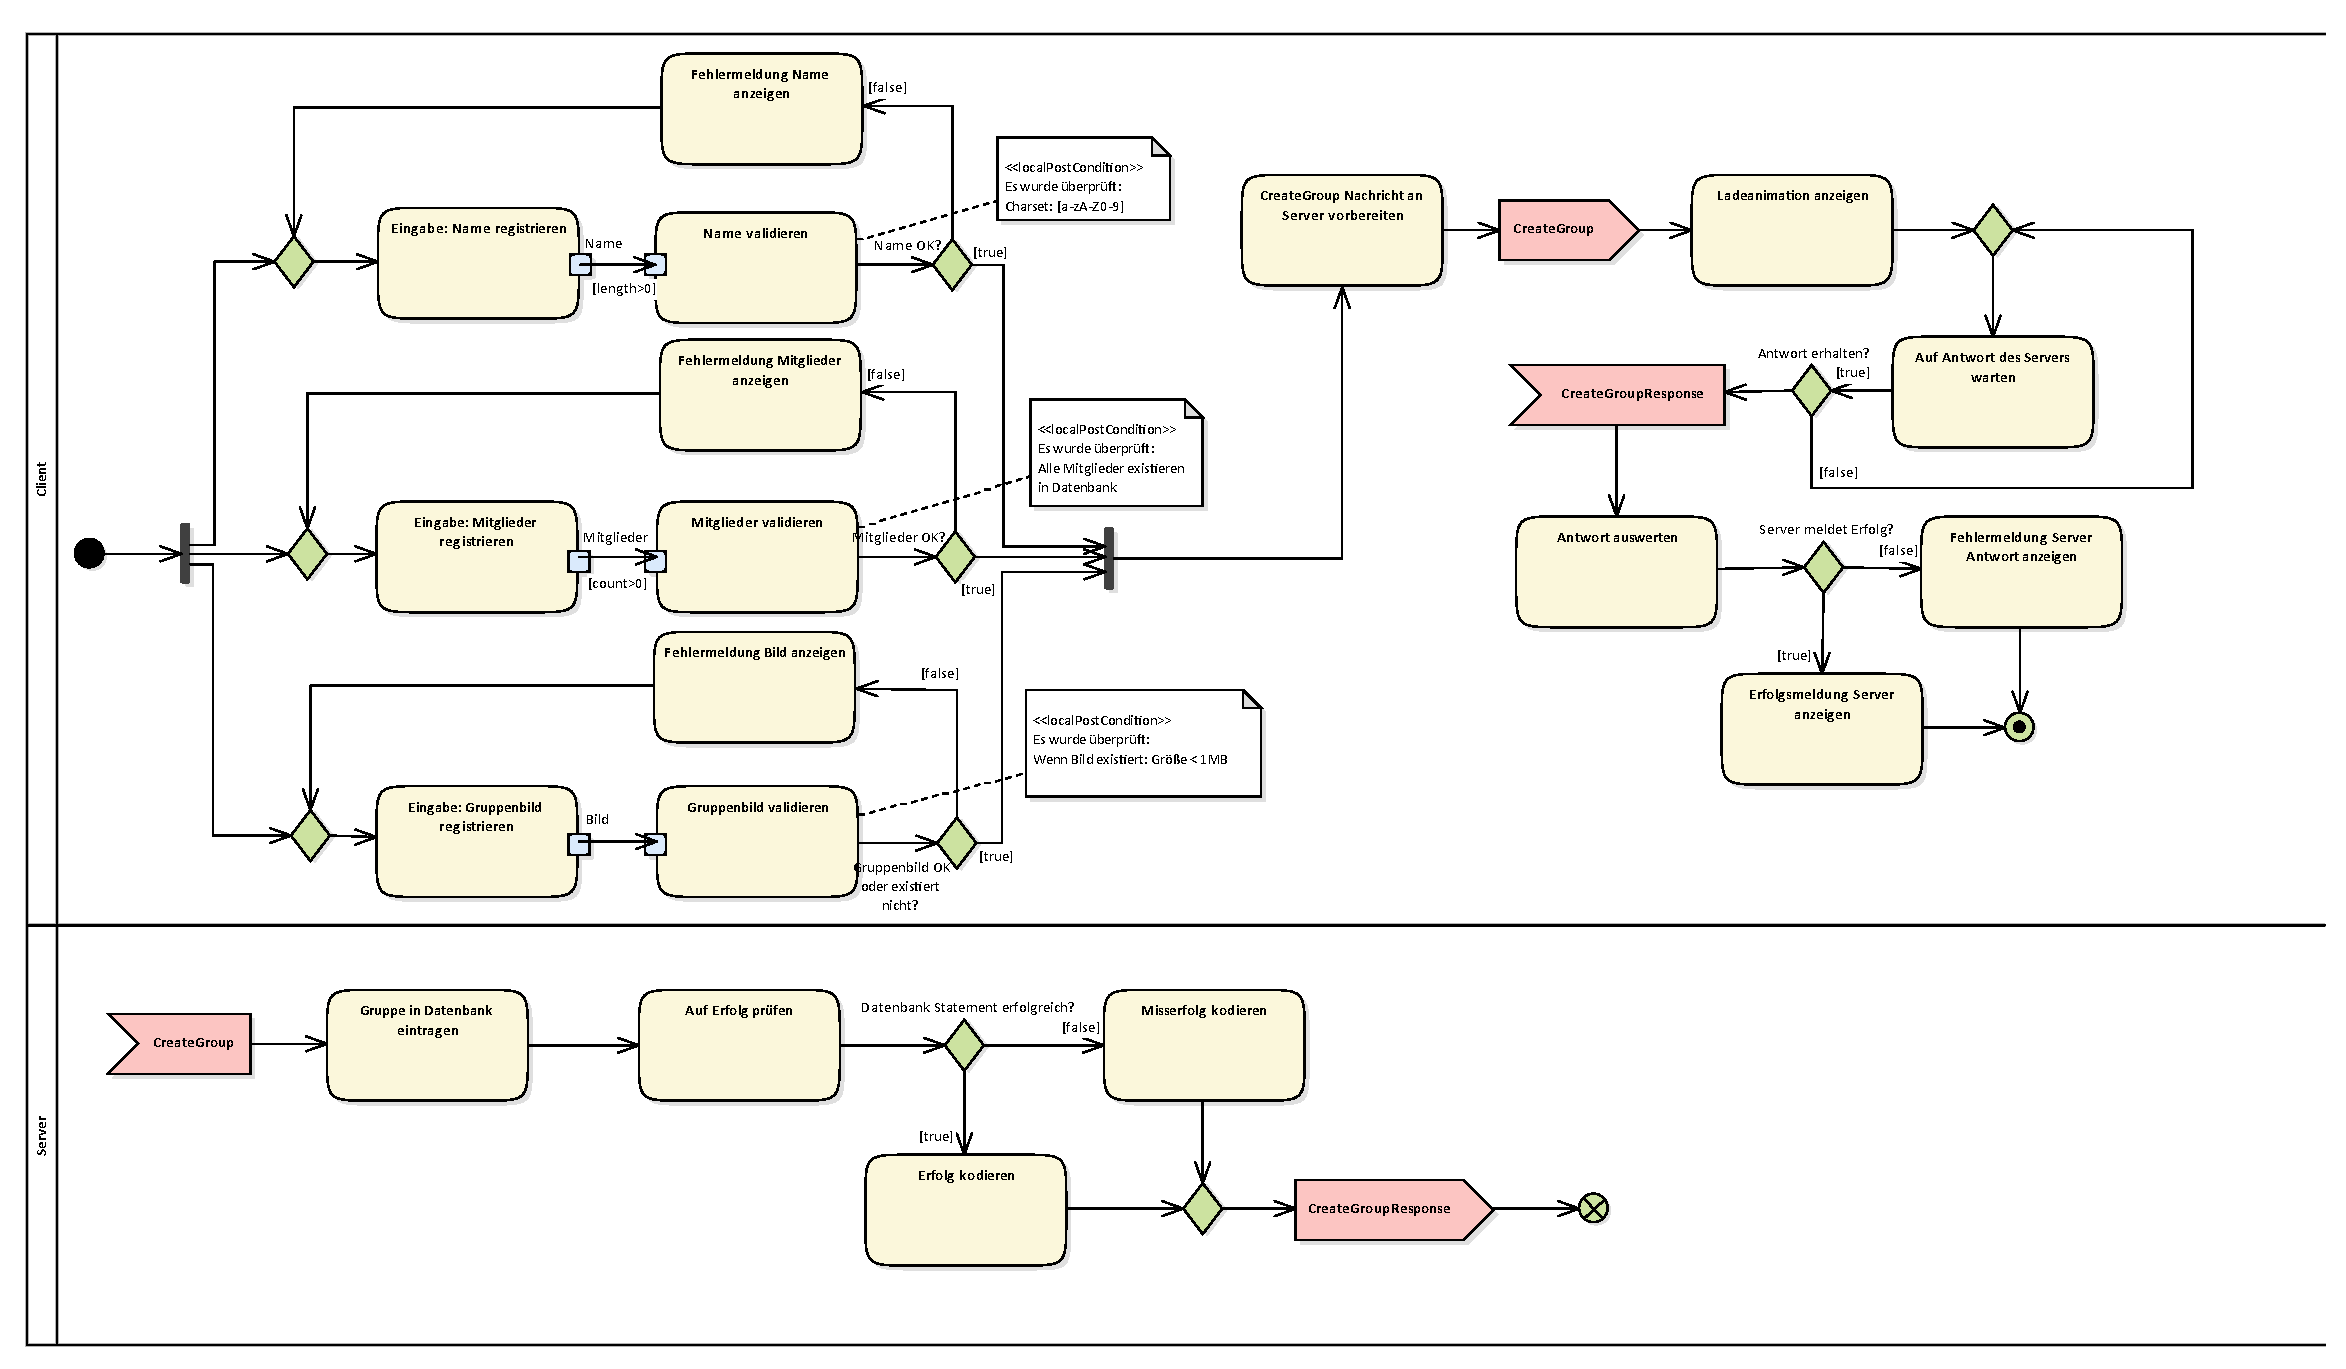
\includegraphics[width=0.9\linewidth]{docs/3_Aktivitaetsdiagramme/Marius/GruppeErstellen.pdf}
	\label{fig:ActDia_Gruppe_Erstellen}
\end{figure}

\vfill
\vfill

\subsection*{Bewerten}
\begin{figure}[h!]
	\centering
	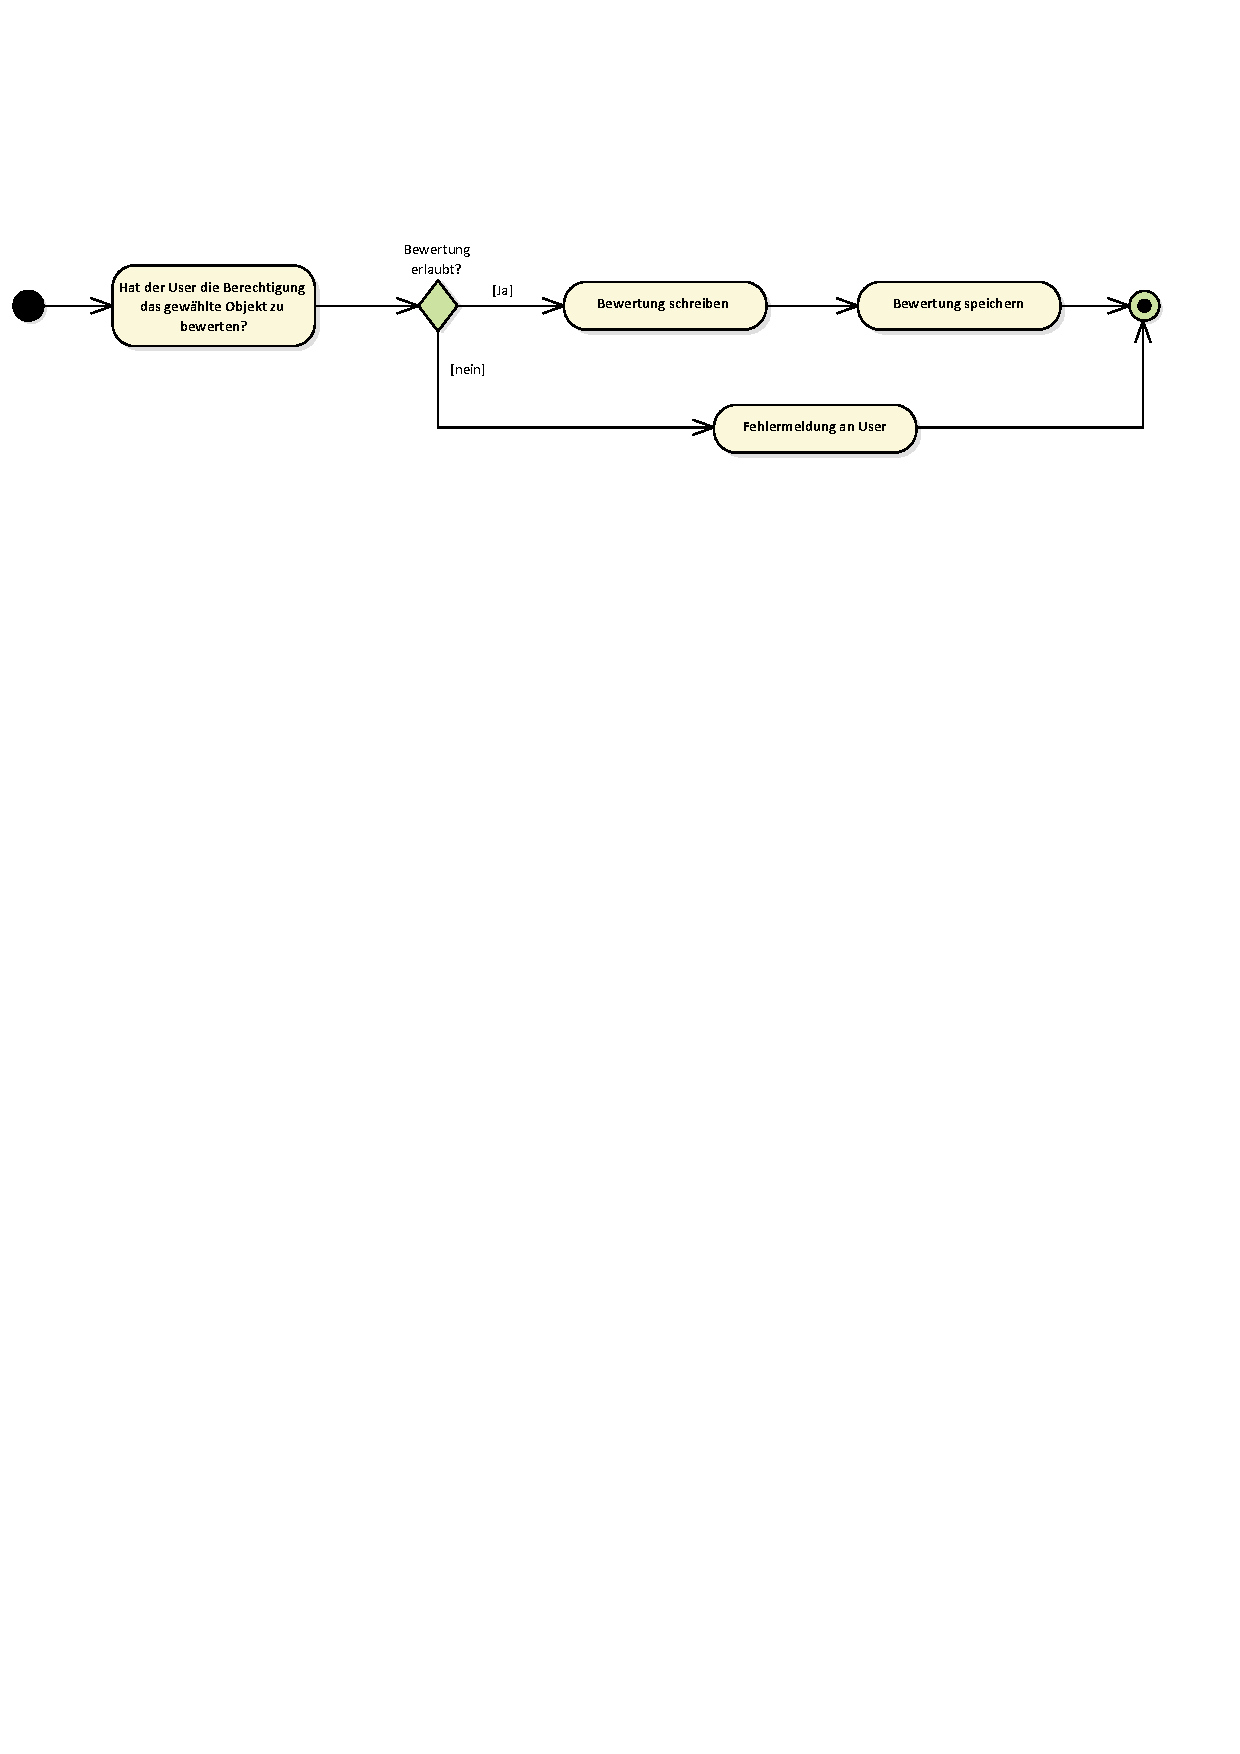
\includegraphics[width=0.8\linewidth]{docs/3_Aktivitaetsdiagramme/Richard/bewerten.pdf}
	\label{fig:ActDia_Bewerten}
\end{figure}

\vfill

\subsection*{Gruppe Verwalten}
\begin{figure}[h!]
	\centering
	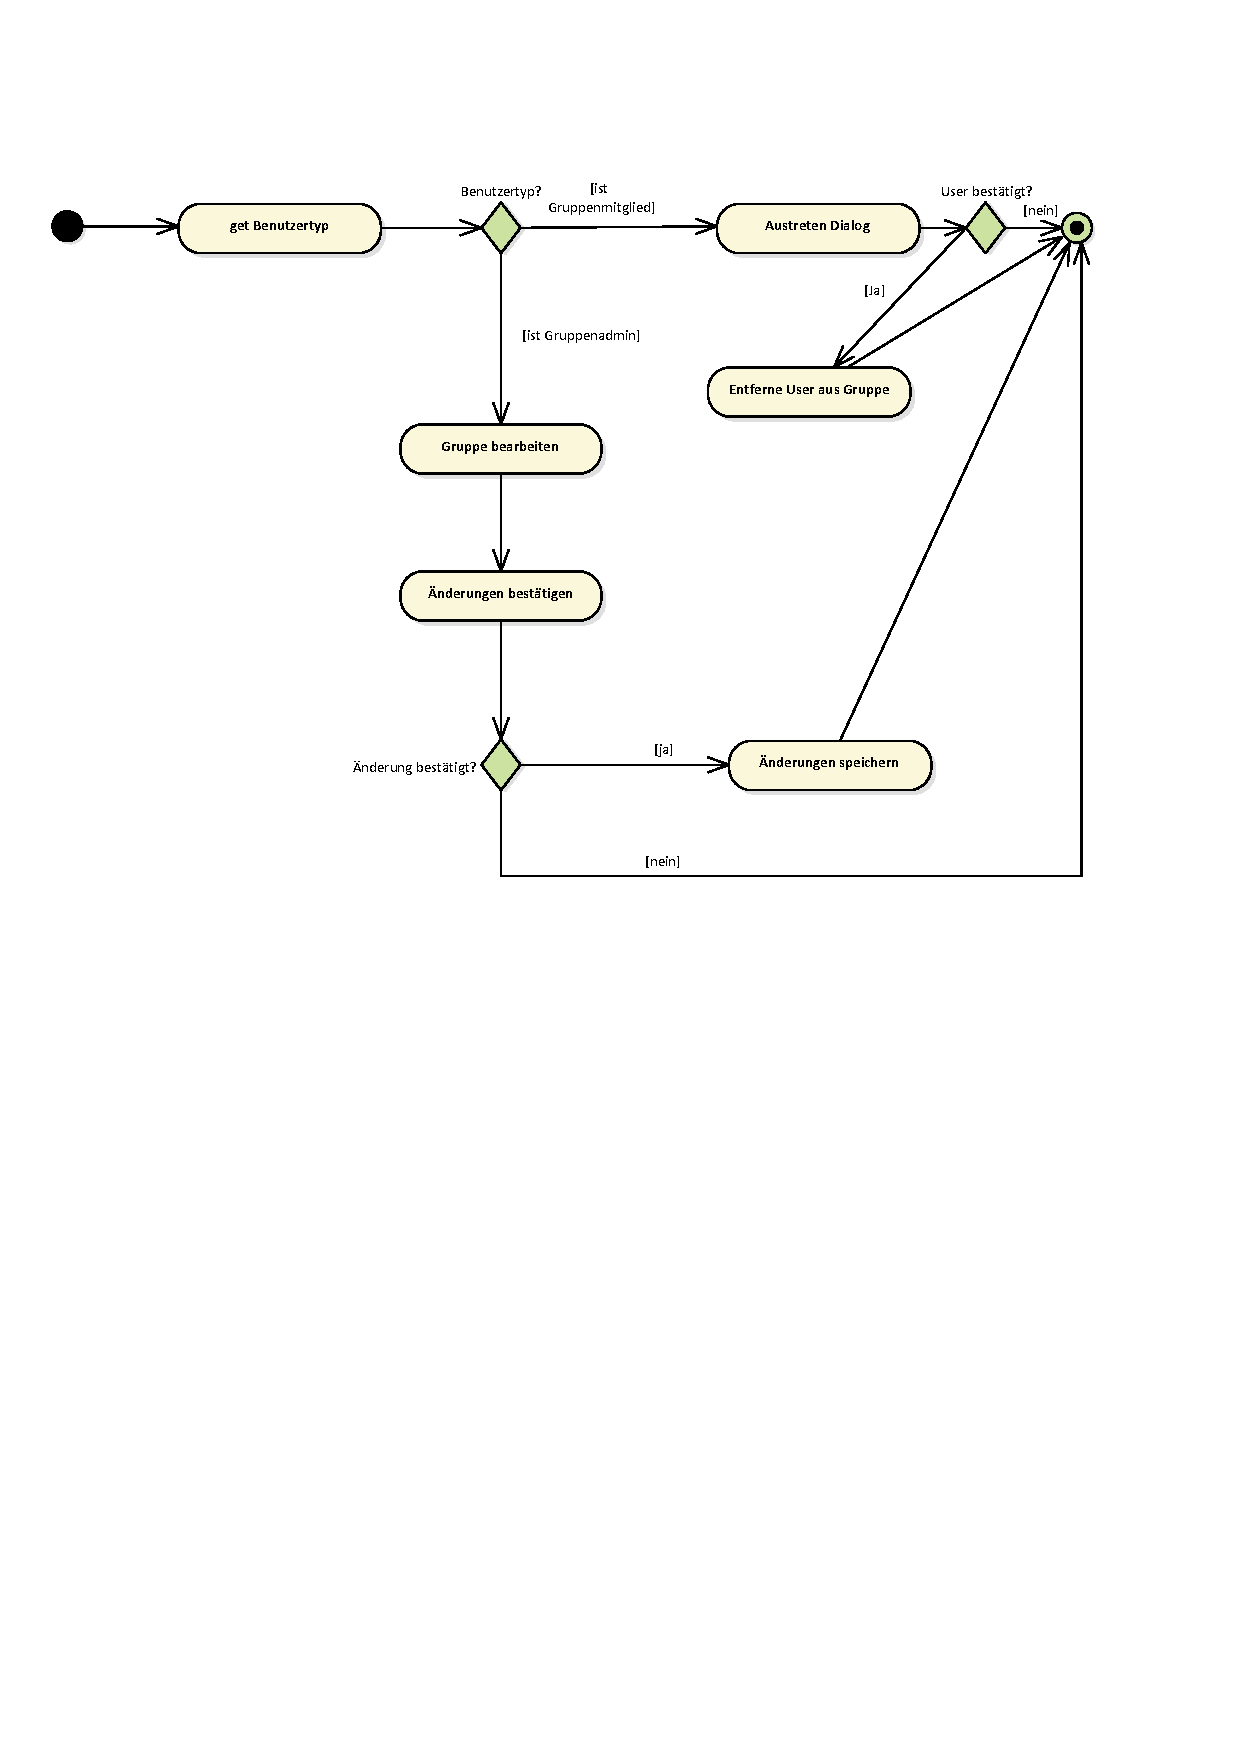
\includegraphics[width=0.8\linewidth]{docs/3_Aktivitaetsdiagramme/Richard/gruppe_verwalten.pdf}
	\label{fig:ActDia_Gruppe_Verwalten}
\end{figure}

\vfill
\pagebreak
\vfill

\subsection*{Chat}
\begin{figure}[h!]
	\centering
	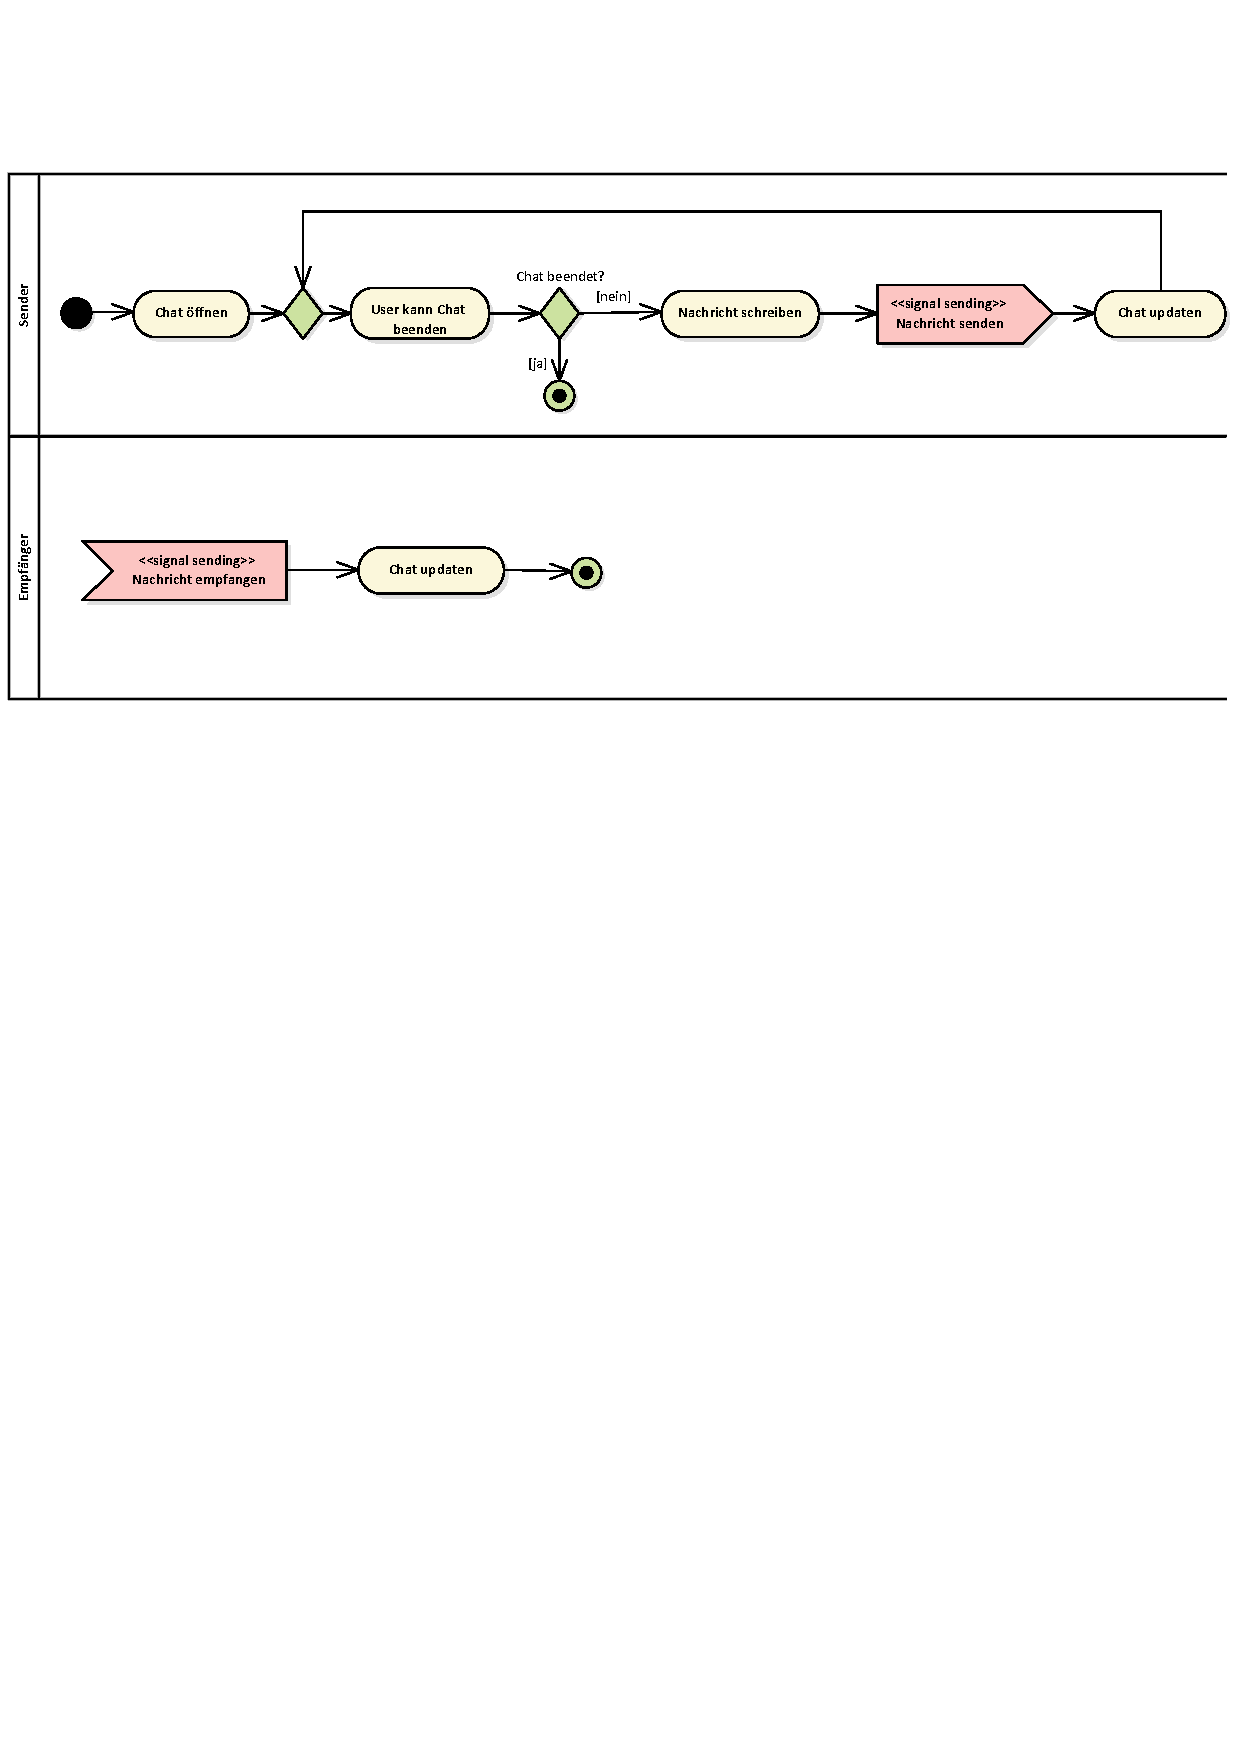
\includegraphics[width=0.8\linewidth]{docs/3_Aktivitaetsdiagramme/Richard/chat.pdf}
	\label{fig:ActDia_Chat}
\end{figure}

\vfill
Eine detailierte Übersicht über die jeweiligen Ersteller der Diagramme ist im \hyperref[app:B_DiagrammUebersicht]{Teil B} des Appendix einzusehen.
\\
\\

\pagebreak

\section{Zustandsdiagramme}

\section{Klassendiagram}

\pagebreak
\section{Sequenzdiagramme}
\subsection*{Anmelden Erfolgreich}
\vfill
\begin{figure}[h!]
	\centering
	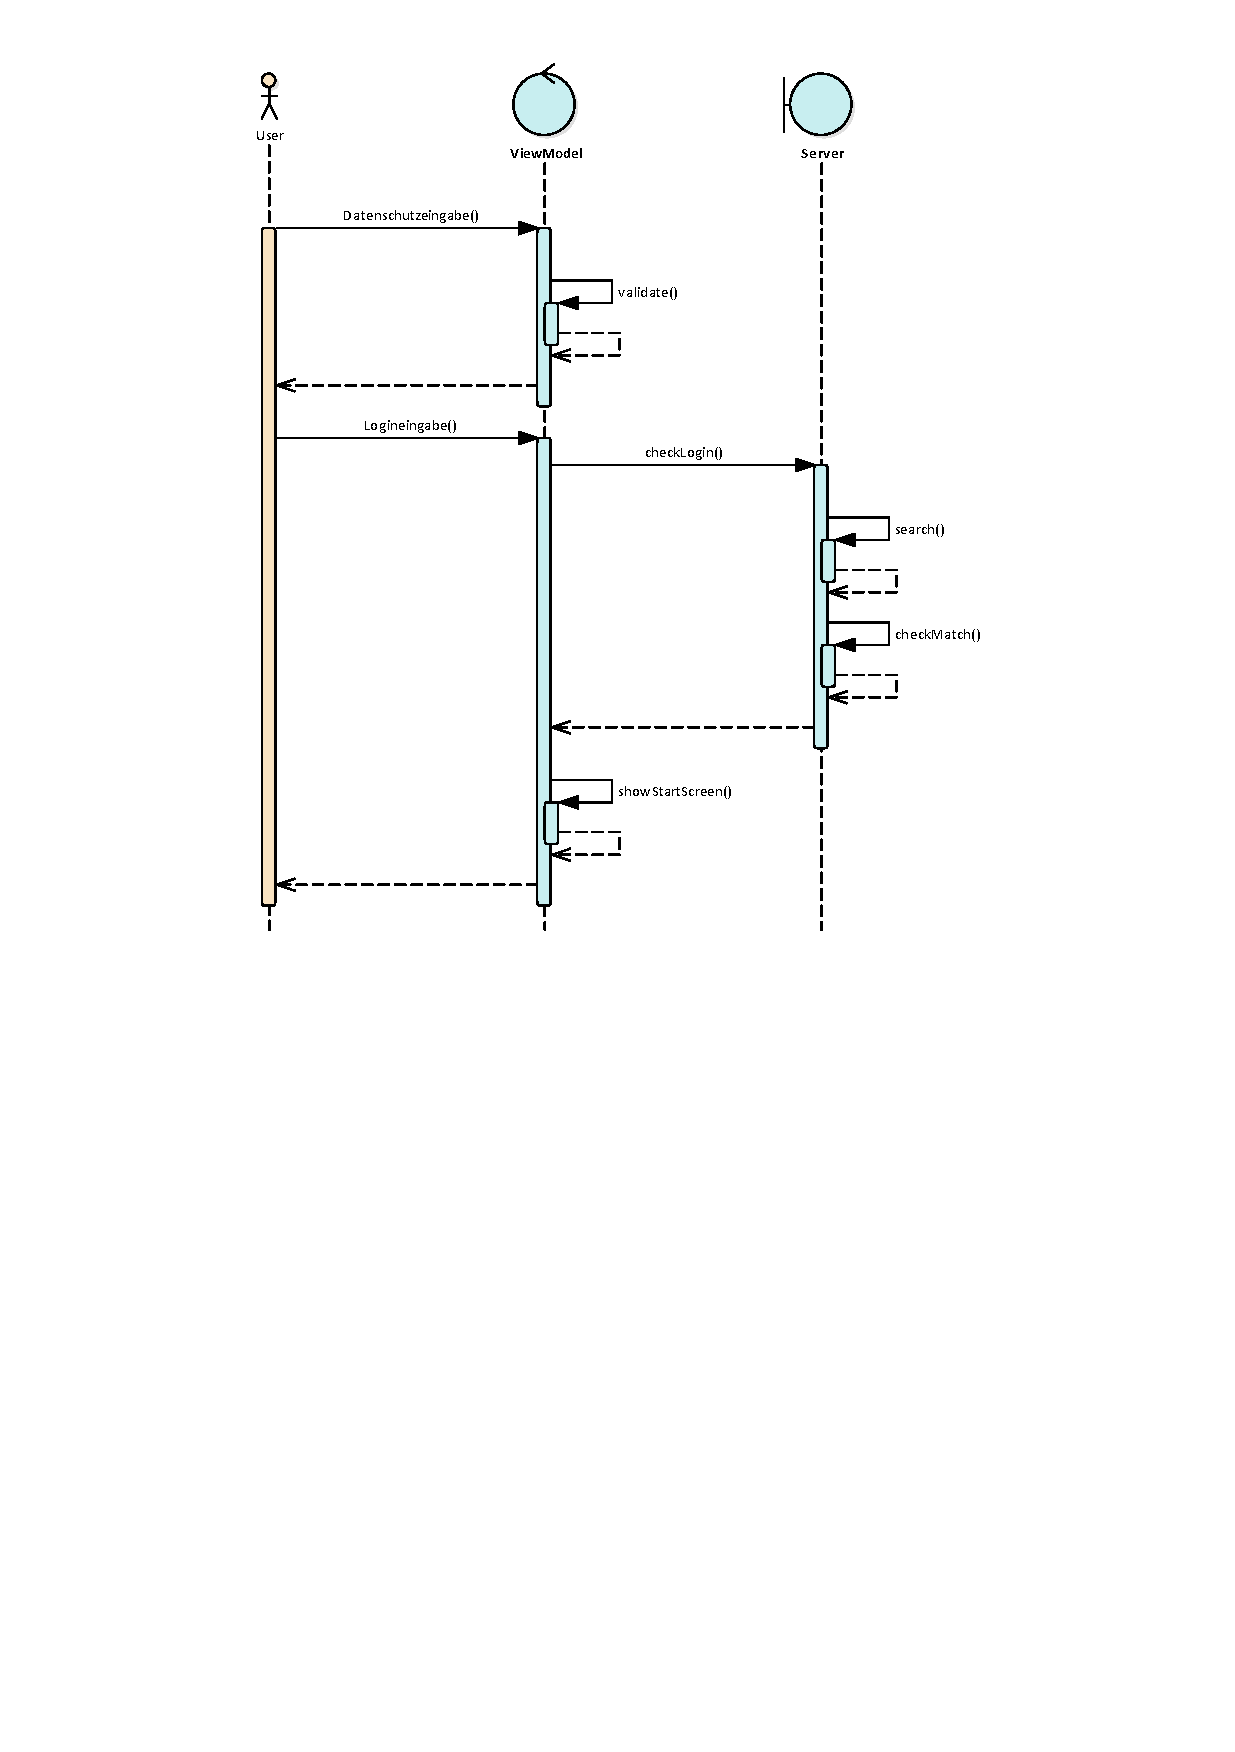
\includegraphics[width = 0.8\linewidth]{docs/6_Sequenzdiagramme/Marius/AnmeldenSuccess.pdf}
	\label{fig:SeqDia_Anmelden_Erfolgreich}
\end{figure}

\vfill
\pagebreak

\subsection*{Anmelden Fehlgeschlagen}
\vfill
\begin{figure}[h!]
	\centering
	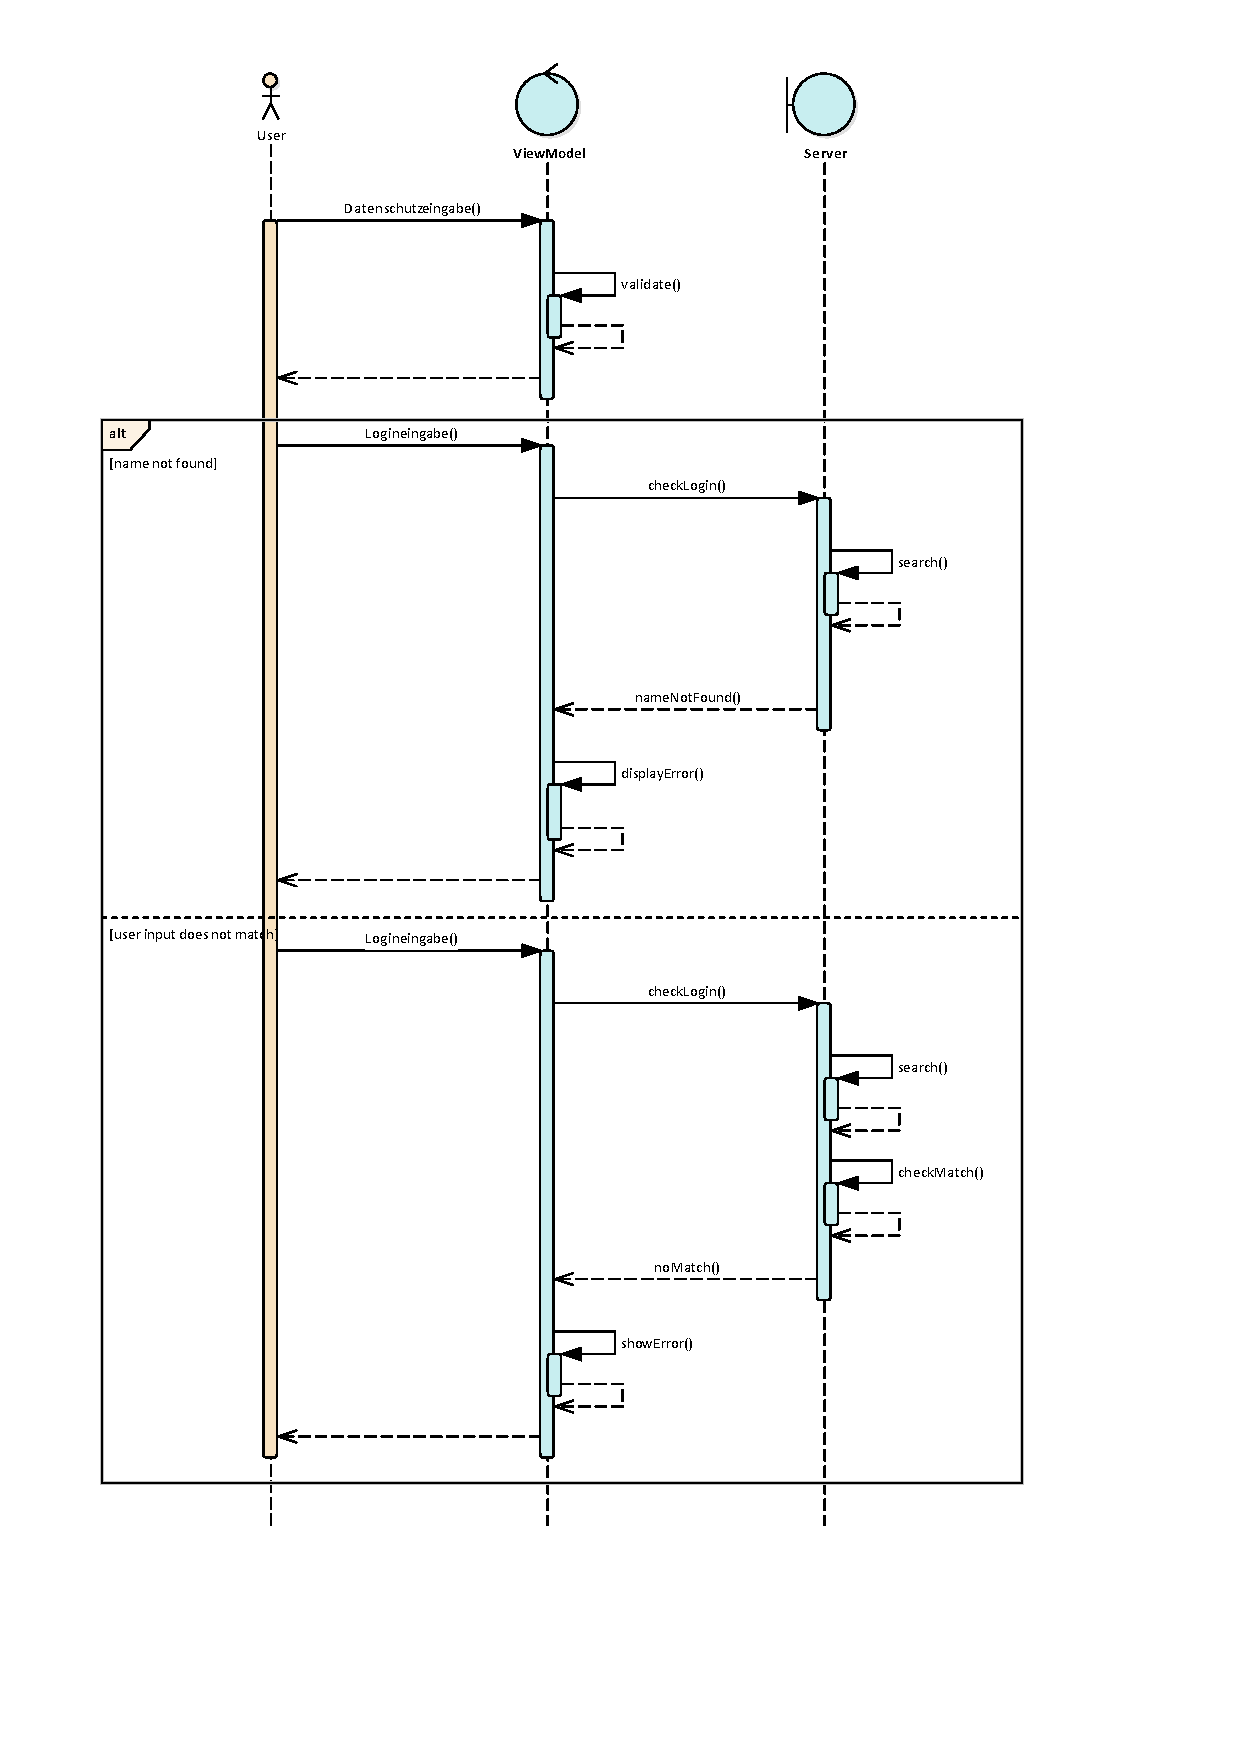
\includegraphics[width = 0.8\linewidth]{docs/6_Sequenzdiagramme/Marius/AnmeldenFailure.pdf}
	\label{fig:SeqDia_Anmelden_Fehlgeschlagen}
\end{figure}

\vfill


%=========APPENDIX==========

\pagebreak
\renewcommand{\appendixtocname}{Appendix}
\renewcommand{\appendixpagename}{Appendix}
\begin{appendices}
	\addtocontents{toc}{\protect\setcounter{tocdepth}{2}}
	\makeatletter
	\addtocontents{toc}{%
		\begingroup
		\let\protect\l@chapter\protect\l@section
		\let\protect\l@section\protect\l@subsection
	}
%	\makeatother

	\section{Personen}
	\label{app:A_Personen}
	\begin{tabularx}{\textwidth}{|l|l|l|X|}
		\hline
		\colorcell{Rolle} & \colorcell{Name} & \colorcell{Telefon} & \colorcell{Email}\\
		\colorcelllight{Projektleitung} & \label{person:MarkusBauer}Markus Bauer &10123 & \mailto{markus.bauer@st.oth-regensburg.de}\\
		\hline
		\colorcelllight{Frontend} & \label{person:MariusTuschl}Marius Tuschl &0114 &\mailto{marius.tuschl@st.oth-regensburg.de}\\
		\hline
		\colorcelllight{Backend} & \label{person:RichardTscharntke}Richard Tscharntke &1269& \mailto{richard.tscharntke@st.oth-regensburg.de}\\
		\hline
		\colorcelllight{Marketinng} & \label{person:PatrickGruber}Patrick Gruber&1337&\mailto{patrick.gruber@st.oth-regensburg.de}\\
		\hline
		\colorcelllight{Anwender} & \label{person:PiaEichinger}Pia Eichinger&0314&\mailto{pia.eichinger@st.oth-regensburg.de}\\
		\hline
		\colorcelllight{Gamemaster}&\label{person:FlorianLoher}Florian Loher&0154&\mailto{florian.loher@st.oth-regensburg.de}\\
		\hline
		\colorcelllight{Forenadmin}&\label{person:FlorianLink}Florian Link&3234&\mailto{florian.link@st.oth-regensburg.de}\\
		\hline
		\colorcelllight{Zahlungsdienst}&\label{person:MrPayPal}Mr.PayPal&9595&\mailto{info@paypal.de}\\
		\hline
		\colorcelllight{Appstore}&\label{person:MrGoogle}Mr.Google&8371&\mailto{info@google.de}\\
		\hline
	\end{tabularx}

	\section{Übersicht Diagrammersteller}
	\label{app:B_DiagrammUebersicht}
	\begin{tabularx}{\linewidth}{|X|X|X|}
		\hline
		\colorcell{Ersteller} & \colorcell{Diagramm-Art} & \colorcell{Diagramm-Name}\\
		\hline
		Patrick Gruber&Aktivitätsdiagramm&\hyperref[fig:ActDia_Profil_Individualisieren]{Profil Individualisieren}\\
		\hline
		Patrick Gruber&Aktivitätsdiagramm&\hyperref[fig:ActDia_Foreneinntrag_Schreiben]{Foreneintrag Schreiben}\\
		\hline
		Patrick Gruber&Aktivitätsdiagramm&\hyperref[fig:ActDia_Forum_Verwalten]{Forum Verwalten}\\
		\hline
		\hline
		Markus Bauer&Aktivitätsdiagramm&\hyperref[fig:ActDia_Listen_Lassen]{Listen Lassen}\\
		\hline
		Markus Bauer&Aktivitätsdiagramm&\hyperref[fig:ActDia_Spieler_Suchen]{Spieler Suchen} \\
		\hline
		Markus Bauer&Aktivitätsdiagramm&\hyperref[fig:ActDia_Termin_Suchen]{Termin Suchen}\\
		\hline
		\hline
		Marius Tuschl&Use Case Diagramm&\hyperref[fig:UCD]{Use Case Diagramm}\\
		\hline
		Marius Tuschl&Systemkontextdiagramm&\hyperref[fig:SystemKontext]{Systemkontext Diagramm}\\
		\hline
		Marius Tuschl&Aktivitätsdiagramm&\hyperref[fig:ActDia_Anmelden]{Anmelden}\\
		\hline
		Marius Tuschl&Aktivitätsdiagramm&\hyperref[fig:ActDia_Registrieren]{Registrieren}\\
		\hline
		Marius Tuschl&Aktivitätsdiagramm&\hyperref[fig:ActDia_Gruppe_Erstellen]{Gruppe Erstellen}\\
		\hline
		Marius Tuschl&Sequenzdiagramm&\hyperref[fig:SeqDia_Anmelden_Erfolgreich]{Anmelden Erfolgreich}\\
		\hline
		Marius Tuschl&Sequenzdiagramm&\hyperref[fig:SeqDia_Anmelden_Fehlgeschlagen]{Anmelden Fehlgeschlagen}\\
		\hline
		\hline
		Richard Tscharntke&Aktivitätsdiagramm&\hyperref[fig:ActDia_Bewerten]{Bewerten}\\
		\hline
		Richard Tscharntke&Aktivitätsdiagramm&\hyperref[fig:ActDia_Gruppe_Verwalten]{Gruppe Verwalten}\\
		\hline
		Richard Tscharntke&Aktivitätsdiagramm&\hyperref[fig:ActDia_Chat]{Chat}\\
		\hline
	\end{tabularx}

	\section{Individuelle Klassendiagramme}
	\label{app:C_Klassendiagramme}
	
	
	\addtocontents{toc}{\endgroup}
\end{appendices}

\end{document}